% \documentclass[a4paper, anonymous, thm-restate]{lipics-v2021}
\documentclass[conference]{IEEEtran}

% \IEEEoverridecommandlockouts
% The preceding line is only needed to identify funding in the first footnote. If that is unneeded, please comment it out.

%\usepackage{lmodern}
%\usepackage[nocompress]{cite}
\usepackage{hyperref}
%% url
\usepackage{url}
%% maths
\usepackage{amsmath,amssymb,amsthm,bm,centernot}
%% \usepackage{amsfonts}
%% \usepackage{amsthm}

%% algorithms
\usepackage{algorithmicx}
\usepackage[ruled, linesnumbered, noend]{algorithm2e}
\usepackage{multicol}

%% images
\usepackage{graphicx}
\usepackage[dvipsnames]{xcolor}
%% inparaenum
\usepackage{paralist}
% \usepackage{todonotes} %% after paralist to avoid clashes
% \newcommand{\note}[1]{\todo[size=\small]{#1}}
% \setlength{\marginparwidth}{2cm}
%% tables
\usepackage{booktabs}
\usepackage{multirow}
%% figures
%\usepackage{caption}
\usepackage{subfig}
\usepackage{tikz}
\usetikzlibrary{decorations.pathreplacing,plotmarks,shapes,matrix}
%% transform eps in pdf crossplateform
\usepackage{epstopdf}
\usepackage{epsfig}

\usepackage{xspace}
\usepackage{pifont}% http://ctan.org/pkg/pifont
\newcommand{\cmark}{\ding{51}}%
\newcommand{\xmark}{\ding{55}}%

\newcommand{\NAME}[0]{\mbox{AS-cast}\xspace}
\newcommand{\NAMEB}[0]{\mbox{S-cast}\xspace}
\newcommand{\NAMEC}[0]{\mbox{xAS-cast}\xspace}
\newcommand{\TODO}[1]{\textcolor{red}{#1}}
\newcommand{\REF}[0]{\textcolor{purple}{REF}\xspace}

\newcommand{\PA}[0]{SkyBlue}
\newcommand{\PB}[0]{BurntOrange}
\newcommand{\PC}[0]{YellowGreen}
\newcommand{\PD}[0]{YellowGreen}
\newcommand{\PX}[0]{SkyBlue}
\newcommand{\PY}[0]{YellowGreen}
\newcommand{\WRONG}[0]{red!75}

\newtheorem{problem}{Problem Statement}
\newtheorem{definition}{Definition}
\newtheorem{lemma}{Lemma}
\newtheorem{theorem}{Theorem}
\newtheorem{corollary}{Corollary}
\newcommand{\eventually}{\Diamond\,}
\newcommand{\ie}{{i.e.,}\xspace}
\newcommand{\eg}{{e.g.,}\xspace}

\newcommand{\process}{node\xspace}
\newcommand{\processes}{nodes\xspace}
\newcommand{\Process}{Node\xspace}
\newcommand{\Processes}{Nodes\xspace}
\newcommand{\node}{\process}
\newcommand{\nodes}{\processes}
\newcommand{\Node}{\Process}
\newcommand{\Nodes}{\Processes}

\title{\NAME: Lock Down the Traffic\\of Decentralized Content Indexing at the Edge}
% \titlerunning{\NAME: Lock Down the Traffic of Decentralized Content Indexing at the Edge}

%% \keywords{
%%   Edge, decentralized content indexing, scoped
%%   broadcast, logical partitioning
%% }

%% \ccsdesc[500]{Networks~Network protocols}

\author{\IEEEauthorblockN{Adrien L{\`e}bre, Brice N{\'e}delec, Alexandre Van Kempen}
  \IEEEauthorblockA{\textit{Inria Rennes}, Nantes, France\\first.last@inria.fr}
}

%% \author{Adrien L{\`e}bre}{Affiliation}{address}{}{} %% anon for now, so w/e
%% \author{Brice N{\'e}delec}{Affiliation}{address}{}{}
%% \author{Alexandre Van Kempen}{Affiliation}{address}{}{}


\begin{document}

% \author{Anonymous}
% \proceedings{}
%\copyright{Adrien l{\'ebre}, Brice N{\'e}delec, Alexandre Van Kempen}

\maketitle


\begin{abstract}
  %% Context and problem
  Although the holy grail to store and manipulate data in Edge
  infrastructures is yet to be found, state-of-the-art approaches
  demonstrated the relevance of replication strategies that bring
  contents closer to consumers: The latter enjoy better response time
  while the volume of data passing through the network decreases
  overall.
  %% Although, there is no major solution to store and manipulate data in
  %% Edge infrastructures yet, existing proposals demonstrated the
  %% relevance of appropriate replication strategies to bring contents
  %% closer to consumers, reducing the impact of the latency as well as
  %% the volume of data passing through the network overall.  
  Unfortunately, locating the closest replica of a specific content
  requires indexing \emph{every live} replica along with its
  \emph{location}.
  %
  %Current proposals built on a centralized service face scalability
  %issues, single point of failure, as well as latency penalities where
  %locating replicas may effectively take more time than actually
  %downloading contents. Instead, data consumer \processes must
  %maintain an up-to-date index themselves. Unfortunately, maintaining
  %an index of all live replicas at every \process would prove overly
  %costly in terms of memory and generated traffic, especially in large
  %scale dynamic systems where \processes create and destroy replicas
  %at any time.
  % 
  Relying on remote services contradicts with the properties of Edge
  infrastructures as locating replicas may effectively take more time
  than actually downloading contents.  At the opposite, maintaining
  such an index at every \process would prove overly costly in terms
  of memory and traffic, especially since \processes can create and
  destroy replicas at any time.
  
  %%% Our proposal
  \noindent In this paper, we abstract content indexing as distributed
  partitioning:
  every \process only indexes its closest replica, and
  connected \processes with similar index compose a partition. Our
  decentralized implementation \NAME
  \begin{inparaenum}[(i)]
  \item is efficient, for it uses partitions to lock down the traffic
    generated by its operations to relevant \processes, yet it
  \item guarantees that every \process eventually acknowledges its
    partition despite concurrent operations.
  \end{inparaenum}
  %% When a \node replicates a content, it notifies all \nodes (new
  %% members of its partition) that are closer from it than any other
  %% replica; When a \node destroys a replica, it notifies members of
  %% its partition to switch to another closer partition. \NAME
  %% guarantees that eventually, every \process knows its best
  %% partition, hence its closest replica, despite concurrent
  %% operations and receipt orders.
  Our complexity analysis supported by simulations shows that \NAME
  scales well in terms of generated traffic and termination time. As
  such, \NAME can constitute the building block of new geo-distributed
  services.
\end{abstract}

%% \begin{IEEEkeywords}
%% Edge infrastructures, decentralized content indexing, scoped
%% broadcast, logical partitioning protocol
%% \end{IEEEkeywords}

%%% Local Variables: 
%%% mode: latex
%%% TeX-master: "../paper"
%%% ispell-local-dictionary: "english"
%%% End: 



\section{Introduction}


\begin{figure*}
\centering
\subfloat[\Process~$R$ efficiently advertises its content using epidemic propagation. Every \process requests $R$ if needed.\label{fig:partition_intuitionA}]{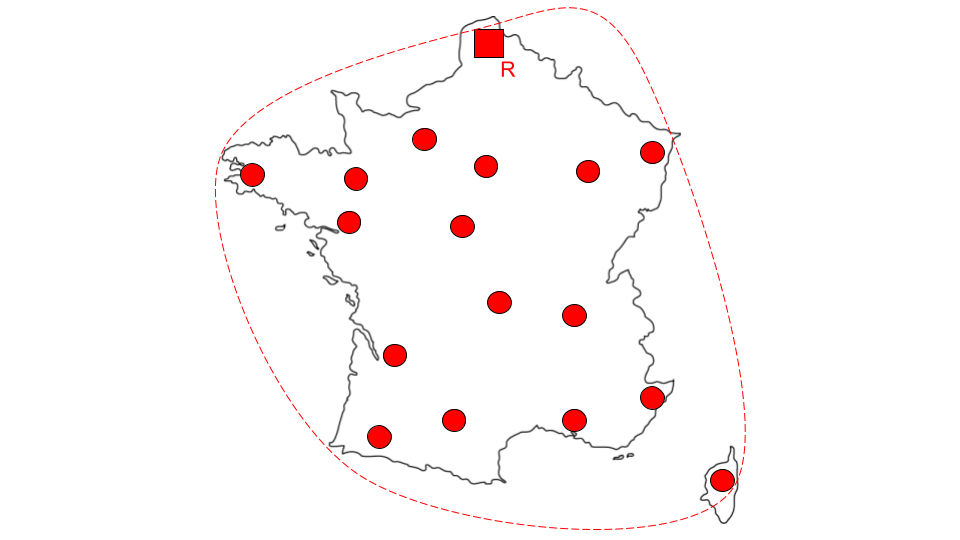
\includegraphics[trim=6cm 0.33cm 6cm 0.33cm, clip, width=0.24\textwidth]{img/Dynamic-partitioning-1.png}}
\hfill
\subfloat[\Process $G$ creates a second replica splitting the red set in two. \Processes request their closest replica host.\label{fig:partition_intuitionB}]{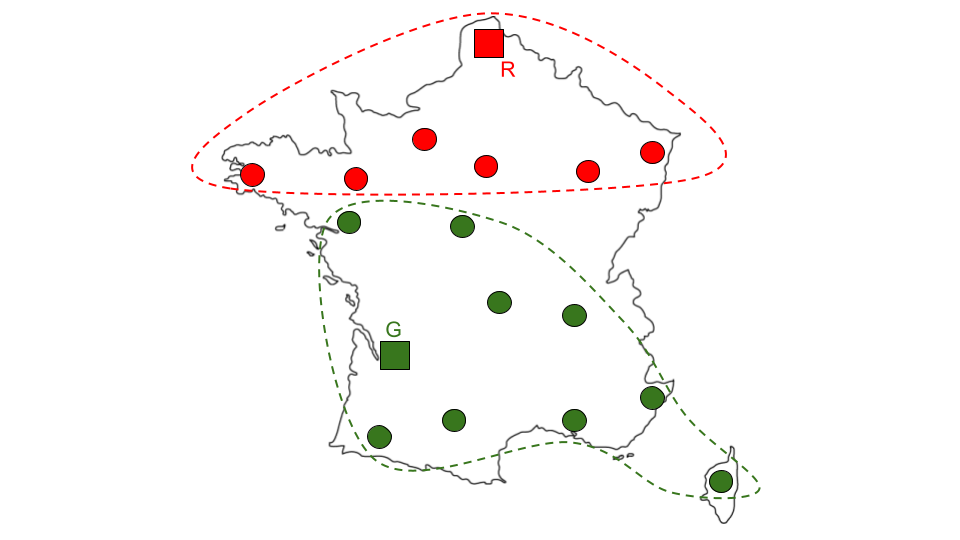
\includegraphics[trim=6cm 0.33cm 6cm 0.33cm, clip, width=0.24\textwidth]{img/Dynamic-partitioning-2.png}}\hfill
\subfloat[\Process $B$ creates another replica. \Process~$B$ needs to notify only a small subset of \processes.\label{fig:partition_intuitionC}]{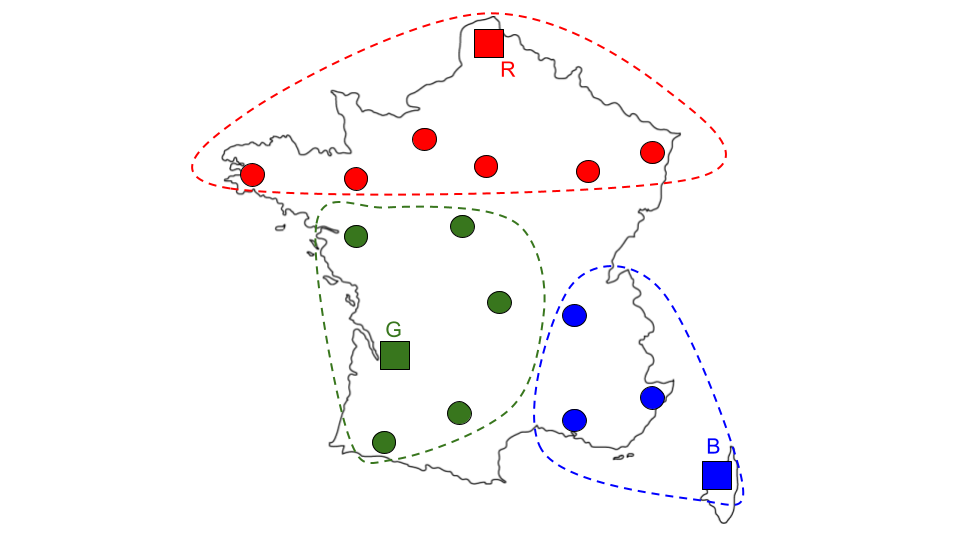
\includegraphics[trim=6cm 0.33cm 6cm 0.33cm, clip, width=0.24\textwidth]{img/Dynamic-partitioning-3.png}}\hfill
\subfloat[\Process $G$ destroys its replica. \Processes that belong to its partition must find the closest partition they are in.\label{fig:partition_intuitionD}]{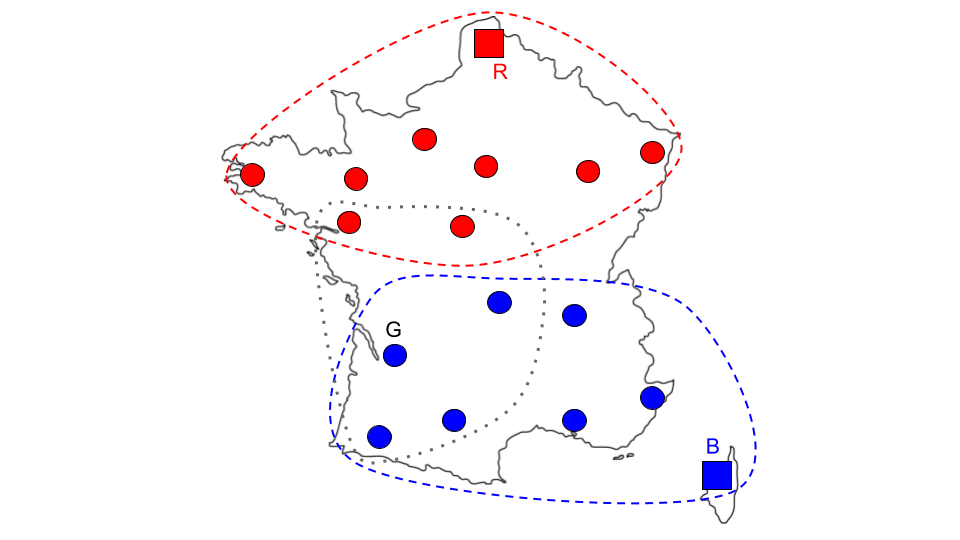
\includegraphics[trim=6cm 0.33cm 6cm 0.33cm, clip, width=0.24\textwidth]{img/Dynamic-partitioning-4.png}}
%
\caption{The french RENATER topology. Partitions
  grow and shrink depending on creations and removals of
  replicas.} \label{fig:partition_intuition}
\end{figure*}

%%% Local Variables: 
%%% mode: latex
%%% TeX-master: "../paper"
%%% ispell-local-dictionary: "english"
%%% End: 
 %% positioning

In recent years, the data storage paradigm shifted from centralized in
the cloud to distributed at the edges of the network. 
% There is an ongoing evolution of storing data from the cloud to the
% edges of the network.
This shift aims at keeping the data close to
\begin{inparaenum}[(i)]
\item its producers since data may be too expensive or sensitive to be
  transmitted through the network; and
\item its consumers so data may quickly and efficiently reach
  them~\cite{cachier, foggy_cache, shi2016edge}.
\end{inparaenum}
%% It avoids transmitting Either because it is where it has been
%% created and it is too expensive to be transmitted through the
%% network, or because it has been replicated to bring data closer to
%% the end users ~\cite{shi2016edge, foggy_cache, cachier}.
%
To favour this transition, new designs for data management across Edge
infrastructures have been investigated~\cite{confais2017object,
  confais2017performance, fogstore, hasenburg2020towards}.  They
enable strategies to confine traffic by writing data locally and
replicating content according to effective needs. However, locating
content remains challenging. Retrieving a content location may
actually take more time than retrieving the content itself.
%% Although
%% these systems, provide good properties such as favouring network
%% traffic confinement by writting data locally and replicating contents
%% according to the effective needs, determining the location where to
%% get the content might be more expensive than retrieving the content
%% itself.
%
Indeed, these systems, when not using a centralized index hosted in a
Cloud~\REF, rely on distributed hash
tables~\cite{maymounkov2002kademlia} spread across the different
\processes composing the infrastructure. When a client wants to access
specific content, it requests a remote \process to provide at least
one \process identity to retrieve this content from. After it
retrieved the content, the client can create another replica to
improve the performance of future accesses, but it must contact the
content indexing service again to notify of such change.
%% a local replica is created to improve the performance for future
%% accesses and the process in charge of maintaining the index is
%% contacted once again to reflect this new location.
%

%This strategy has two majors drawbacks :
%\begin{itemize}
%  \item (i) the lookup penalty: the network latency to reach this
%    remote node incurs an additional delay~\cite{asrese2019measuring,
%      doan2019tracing} to get the object before
%    being able to start its downloading ;
%  \item (ii) the selection of the node(s) from which the content is
%    returned: due to the lack of information that would allow the  a request to each process storing a
%%    replica is perfomed in
%\end{itemize}

These approaches directly contradict with the objectives of Edge
infrastructures that aim at reducing the impact of latency as well as
the volume of data passing through the network.
%
First, accessing a remote \node to request content location(s) raises
hot spots and availability issues. But most importantly, it results in
additional delays that occur even before the actual download
started~\cite{asrese2019measuring, doan2019tracing}.
%
Second, the client gets a list of content locations at the discretion
of content indexing services. Without information about these
locations, it often ends up downloading from multiple replica hosts,
yet only keeping the fastest answer~\REF. In turns, clients either
waste network resources, or face lower response time.
%% there is no information to select the ``best'' node among the
%% possible candidates from which the content could be retrieved. In
%% most cases, this results in parallel requests performed by the
%% client node to each candidate with the goal of retrieving the
%% content as efficient as possible.

To tackle aforementioned limitations, every \process that might
request or replicate content must also host its own content indexing
service in a fully decentralized fashion~\cite{kermarrec2015want}. At
any time, it can immediately locate the closest replica of specific
content.  A naive approach would be that every \process indexes and
ranks \emph{every live} replica along with its \emph{location}
information. When creating or destroying a replica, a \process would
notify all other \processes by efficiently broadcasting its
operation~\cite{birman1999bimodal, hadzilacos1994modular,
  raynal2013distributed}. Unfortunately, this also contradicts with
Edge infrastructure objectives, for such protocol does not confine the
traffic generated to maintain its indexes. A \process may acknowledge
the existence of replicas at the other side of the network while there
already exists a replica next to it.

Instead, a \process creating a replica should notify all and only
\processes that have no closer replica in the system. This would
create interconnected sets of \processes, or \emph{partitions},
gathered around a \emph{source} being their respective replica. A
\process deleting its replica should notify all members of its
partition so they can rally their current closest partition. A
periodic advertisement protocol already provides both these operations
for routing purposes~\cite{hemmati2015namebased}. However, its
functioning requires
\begin{inparaenum}[(i)]
\item to generate traffic even when the system is quiescent, and
\item to finely tune physical-time-based intervals that depend on
  network topology parameters such as network diameter.
\end{inparaenum}

%% A ``simple'' way to tackle the aforementioned limitations would be to
%% maintain on each node composing the infrastructure and for each
%% content, an index of all replicas (and their ``distance'').  In such
%% an approach, each time a new replica is created or deleted, a message
%% is broadcasted from the node that performed the operation (\ie the
%% source) to all nodes, increasing the distance information at each hop.
%% %
%% In addition to being complicated for large-scale systems, maintaining
%% a global view on each node is useless as there is no interest to
%% inform a node of the creation/removal of a replica at the opposite of
%% the network (each node trying to get content from the ``closest''
%% one).  In other words, the broadcast should be limited to a partition
%% of the infrastructure, (\ie the subset of nodes that has to update the
%% current location for this particular content). Obviously, these
%% partitions depend and evolve according to concurrent operations made
%% by nodes (replica creation/removal) as well as dynamic changes in the
%% infrastructure (network failures, node apparitions/leaves).

In this paper, we first define scoped broadcast has a communication
primitive that allows epidemic dissemination of messages as long as
receiving \processes verify an application-dependant predicate.

\noindent Then, we propose \NAME, a logical partitioning protocol that
uses \underline{s}coped broad\underline{cast} to \underline{a}dapt its
partitions, \ie scopes, to creations and deletions of partitions in
the system. Each source advertises its existence to all possibly
interested \processes, \ie only interconnected \processes of its
partition plus \processes bordering its partition. In turns, \NAME
scales well to the number of sources since the higher the number of
partitions, the earlier the dissemination of notifications stops.
%
%% In this paper, we propose a first implementation of such a protocol.
%% Entitled Adaptive Scoped broadcast (\NAME), 
%% our protocol relies on a primitive that forwards
%% messages until a certain condition is reached, \ie the scope. The
%% scope is defined by a boolean function (predicate) that returns
%% whether a message should be propagated or not around its
%% broadcaster. In the current scenario, the stop condition is related to
%% the distance to the nearest replica : if the message that a node receives
%% indicates a content has a longer distance than that which the node
%% knows then the transfer of the message is useless and so stopped.
%

\noindent In addition, \NAME guarantees that despite concurrent
operations, every \process eventually knows one, and only one, source:
its closest. \NAME being reactive, when the system becomes quiescent,
\processes do not require further communications.
%% This primitive is used to guarantee that eventually, every node knows
%% its best partition, hence its closest replica, despite concurrent
%% events and receipt orders. Overall, \NAME is a wait-free reactive protocol for
%% dynamic logical partitioning.  Its overhead actually depends on
%% its operations and current partitions in the system. When the system
%% becomes quiescent, nodes eventually converge to their respective
%% partition and do not require further communication afterward.
% \TODO{talk about the proof}

\noindent Simulations empirically support our complexity analysis and
the scalability of \NAME in large scale networks comprising 10k
\processes. Our experiments also highlight the relevance of \NAME in
autonomous systems. \NAME would allow to lock down the traffic
generated by content indexing, even in contexts where \emph{physical}
partitioning may occur.

\noindent In that regard, \NAME can constitute the building block of
new geo-distributed services.

%% We evaluated our protocol through two simulation scenarios using
%% \textit{Peersim}~\cite{montresor2009peersim}. First, we confirm that
%% \NAME allow consistent partitioning in an ad-hoc network composed of
%% 10K nodes.  Second, we illustrate how \NAME enables the lock down of
%% the traffic in dynamic inter autonomous systems.  More precisely, we
%% simulated a worldwilde infrastructure by duplicating the GEANT
%% topology - a real infrastructure spanning across Europe – and by
%% connecting these two clusters with a high latency link: 200 ms
%% simulating cross-continental communications such as Europe-America.

The rest of this paper is organized as
follows. Section~\ref{sec:background} illustrates the motivation and
problem behind our proposal.  Section~\ref{sec:adaptive} describes
dynamic consistent partitioning and its implementation along with its
complexity. Section~\ref{sec:experimentation} presents our
evaluations.  Section~\ref{sec:related_work} reviews related
work. Finally, Section~\ref{sec:conclusion} concludes and discusses
future work.
  

%%% Local Variables: 
%%% mode: latex
%%% TeX-master: "../paper"
%%% ispell-local-dictionary: "english"
%%% End: 


\section{Background and motivation}
\label{sec:background}

Fog infrastructures are distributed systems comprising heterogeneous
machines interconnected by communication links.

\begin{definition}[Fog infrastructure]
  A fog infrastructure is a \underline{g}raph $G(V, E)$ of
  \underline{v}ertices $V$ and bidirectional \underline{e}dges $E \in
  V \times V$. Edges have symmetric \underline{w}eights $w_{ij} =
  w_{ij}$ with $i, j \in V$.
\end{definition}

\begin{definition}[Logical partitions]
  A logical \underline{p}artition $P_s$ originated at a
  \underline{s}ource process $s \in V$ is a set of interconnected
  processes that do not belong to another logical partition.
\end{definition}


\TODO{Multiple destinations shortest path \REF}.

\begin{algorithm}
  \SetKwProg{Function}{func}{}{}

\small

\DontPrintSemicolon
\LinesNumbered

$O_p$, $W_p$\tcp*[r]{set of neighbors and weights}
$s \leftarrow \varnothing$ \tcp*[r]{best source of partition ($\sigma$)}
$d \leftarrow \infty$ \tcp*[r]{smallest distance to $s$ ($\sigma$ and $\mu$)}


\BlankLine

\Function{\textup{Add ( )} \tcp*[f]{$\alpha_p^0$}} {
  \textup{receiveAdd($\varnothing$, $p$, $0$)} \label{line:lowestbound} \tcp*[f]{$b_p(\alpha_p^0)$}
}

\BlankLine

\Function{\textup{receiveAdd($q$, $s'$, $d'$)} \tcp*[f]{$r_p(\alpha_{s'}^{d'})$ from $q$}} {
  \If (\tcp*[f]{($\phi$)}){$d' < d$} {
      $s \leftarrow s'$ \tcp*[r]{\smash{$d_p(\alpha_{s'}^{d'})$}}
      $d \leftarrow d'$ \;

      \ForEach(\tcp*[f]{\smash{$f_p(\alpha_{s'}^{d'})$}}) {$n \in O_p \setminus q$} {
          \textup{send$_n$($s', d' + W_{pn}$)} \label{line:accumulator}
          \tcp*[r]{\smash{$s_{pn}(\alpha_{s'}^{d'+w_{pn}})$}}
       }      
  }
}

%% \BlankLine

%% \Function{\textup{edgeUp($q$)} \tcp*[f]{new link to $q$}} {
%%   \lIf { $d < \infty$} {\textup{send$_q$($s, d + W_{pq}$)}}
%% }



  \caption{\label{algo:add}Adding partitions by Process $p$.}
\end{algorithm}

Algorithm~\ref{algo:add} shows the instructions of dynamic
partitioning where the only operation available to processes is the
adding of a partition.  Line~\ref{line:lowestbound} shows the lowest
bound. Line~\ref{line:accumulator} shows the accumulator.

\TODO{Removing partition is more difficult.}


%%% Local Variables: 
%%% mode: latex
%%% TeX-master: "../paper"
%%% ispell-local-dictionary: "english"
%%% End: 



\section{Adaptive scoped broadcast}
\label{sec:adaptive}

To provide lazy and dynamic logical partitioning in dynamic networks
using scoped broadcast, all live \processes must collaborate to
disseminate messages that notify new or removed sources to all and
only interested \processes. This section reviews step-by-step the
properties that allow \processes to converge to the desired state
together. It first defines scoped broadcast, then uses it to guarantee
consistent partitioning when a \process can only become a new source
in the system. It highlights the issue when a \process can also remove
its status of source. It shows that using local knowledge and scoped
broadcast, \processes can still reach dynamic consistent partitioning
when they are able to detect possible blocking conditions in the
dissemination of required notifications. Finally, it further constrain
the system by allowing only subsets of \processes to reach lazy
consistent partitioning. This improvement only requires \processes to
know which of their neighbors belong to their own network.

\subsection{Scoped broadcast}
\label{subsec:scoped}

In this paper, we consider Edge infrastructures as a set of
interconnected autonomous systems comprising heterogeneous \nodes
interconnected by communication links. \Processes involved in the
management of content may crash but are not byzantine.  \Processes can
reliably communicate through asynchronous message passing to other
known \processes called neighbors.  We define scoped broadcast as a
communication primitive that propagates a message around its
broadcaster within an application-dependant scope.

\begin{definition}[Autonomous systems]
  An autonomous system is a network comprising nodes and communication
  links that we represent as a \underline{g}raph of
  \underline{v}ertices and \underline{e}dges:
  $G = \langle V, E \rangle$ with $E \in V \times V$. A
  \underline{p}ath $\pi_{xz}$ from \Process~$x$ to \Process~$z$ is a
  sequence of contiguous edges
  $[\langle x, y_1 \rangle, \langle y_1, y_2\rangle, \ldots, \langle
  y_n, z \rangle]$.
\end{definition}

\begin{definition}[\label{def:scoped}\underline{S}coped broad\underline{cast} (\NAMEB)]
  When \Process~$x$ scoped \underline{b}roadcasts $b_x(m)$ a
  \underline{m}essage $m$, every correct \process $y$ within a scope
  \underline{r}eceives $r_y(m)$ and \underline{d}elivers it
  $d_y(m)$. The scope depends on the \underline{s}tate $\sigma$ of
  each \process, the \underline{m}etadata $\mu$ piggybacked by each
  message, and a \underline{p}redicate $\phi$ verified from \process
  to \process:
  $(b_x(m) \wedge r_y(m)) \implies \exists \pi_{xy}: \forall z \in
  \pi_{xy}, \phi(\mu_z, \sigma_z)$.
\end{definition}

This definition encompasses more specific definitions of related
work~\cite{hsiao2005scoped, lue2006scoped, wang2015prodiluvian}. It
underlines the transitive relevance of messages. It also highlights
that the functioning of epidemic propagation is well-aligned with the
objectives of scoped broadcast. As consequence, we assume
implementations relying on the forwarding of messages from
neighbor-to-neighbor.

\begin{definition}[\label{def:forwarding}Forwarding]
  A \process $x$ \underline{f}orwards a message $m$ by
  \underline{s}ending it to its neighbors with metadata that depends
  on its local knowledge: $f_x(m) \implies \forall \langle x, y\rangle
  \in E: s_{xy}(m \oplus \sigma_x)$.
\end{definition}

We use scoped broadcast to efficiently modify the state of each
\process depending on the partitions that exist in the system.



\subsection{Consistent partitioning}
\label{subsec:consistent}

At any time, a \process can decide to become a \emph{source}, hence
creating a new partition in the system by executing an \texttt{Add}
operation. This partition includes at least its source plus
neighboring \processes that are closer to this source than any other
one. Such a distance (or \emph{weight}) is application-dependant: in
the context of maintaining distributed indexes, this would be about
link latency that \nodes could monitor by aggregating \texttt{ping}s;
or operational costs when dealing with multiple tenants.


\begin{figure*}
  \newcommand{\SCALE}{0.95} %% scale of sub figures
  \newcommand\X{50pt}
  \newcommand\Y{-50pt}
  
  \newcommand{\SMSG}{\tiny} %% font size of messages
  \newcommand{\OACK}{0.5} %% opacity of acknowledgement alpha messages

  \newcommand{\LEFT}{\triangleleft}
  \newcommand{\RIGHT}{\triangleright}
  
  \thickmuskip=0mu %% to remove annoying math spacing from caption
  \medmuskip=0mu
  \thinmuskip=0mu
  \begin{center}
    \subfloat[Part A][\label{fig:addA}Both $a$ and $d$
      become sources.  $w_{ab} = 2$; $w_{bc} = w_{bd} = 1$; $w_{cd} =
      3$.]  {
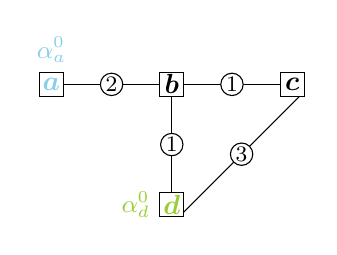
\begin{tikzpicture}[scale=0.87]

  \thickmuskip=0mu
  \medmuskip=0mu
  \thinmuskip=0mu
  
  \newcommand\X{50pt}
  \newcommand\Y{-50pt}

  \newcommand\ADD{\alpha}


  
  \draw (-\X + 5pt, 0) --
  node[shape=circle, draw, fill=white, inner sep=0.5pt, font=\footnotesize]{2}
  (0 - 5pt, 0); %% a - b

  \draw (0 +5pt, 0) --
  node[shape=circle, draw, fill=white, inner sep=0.5pt, font=\footnotesize]{1}
  (\X -5pt, 0); %% b - c
  
  \draw (0, 0 - 5pt) --
  node[shape=circle, draw, fill=white, inner sep=0.5pt, font=\footnotesize]{1}
  (0, \Y + 5pt); %% d - b
  
  \draw (\X + 3pt, 0 - 5pt) --
  node[shape=circle, draw, fill=white, inner sep=0.5pt, font=\footnotesize]{3}
  (0 + 5pt, \Y - 3pt); %% c - d


  
  \draw[fill=white] (-\X, 0) node[color=\PA]{$\bm{a}$} +(-5pt, -5pt) rectangle +(5pt, 5pt);  
  \draw[fill=white] (0, 0) node{$\bm{b}$} +(-5pt, -5pt) rectangle +(5pt, 5pt);
  \draw[fill=white] (\X, 0) node{$\bm{c}$} +(-5pt, -5pt) rectangle +(5pt, 5pt);
  \draw[fill=white] (0, \Y) node[color=\PD]{$\bm{d}$} +(-5pt, -5pt) rectangle +(5pt, 5pt);
  
  \draw (-\X, 5pt) node[above, font=\small, color=\PA]{$\ADD_a^0$};
  \draw (-5pt, \Y) node[left, font=\small, color=\PD]{$\ADD_d^0$};

\end{tikzpicture}
}
    \hspace{1pt}
    \subfloat[Part B][\label{fig:addB}Messages transit through %communication
      links and carry increasing weights.]{
\begin{tikzpicture}[scale=\SCALE]

  \thickmuskip=0mu
  \medmuskip=0mu
  \thinmuskip=0mu
  
  \newcommand\X{50pt}
  \newcommand\Y{-50pt}

  \newcommand\ADD{\alpha}


  
  \draw (-\X + 5pt, 0) --
  node[above=-0.3em, left=-0.3em, above left, font=\tiny]{$\textcolor{\PA}{\ADD_a^2} \rightarrow$}
  (0 - 5pt, 0); %% b - a 

  \draw (0 +5pt, 0) --
  (\X -5pt, 0); %% c - b

  \draw[opacity=0] (0, 0 - 5pt) --
  % node[opacity=1, above=-0.3em, font=\tiny, sloped]{$\textcolor{\PA}{\ADD_a^{3}} \rightarrow$}
  (0, \Y + 5pt); %% b - d
  \draw (0, \Y + 5pt) --
  node[above=-0.3em, font=\tiny, sloped]{$\textcolor{\PD}{\ADD_d^1} \rightarrow$}
  (0, 0 - 5pt);  %% d - b
  
  \draw (\X + 3pt, 0 - 5pt) --
  node[above=-0.3em, sloped, font=\tiny]{$\textcolor{\PD}{\ADD_{d}^{3}} \rightarrow$}
  (0 + 5pt, \Y - 3pt); %% c - d



  \draw[fill=white] (-\X, 0)
  node[color=\PA]{$\bm{a}$}
  +(-5pt, -5pt) rectangle +(5pt, 5pt);  
  \draw[fill=white] (0, 0) node{$\bm{b}$} +(-5pt, -5pt) rectangle +(5pt, 5pt);
  \draw[fill=white] (\X, 0) node{$\bm{c}$} +(-5pt, -5pt) rectangle +(5pt, 5pt);
  \draw[fill=white] (0, \Y) node[color=\PD]{$\bm{d}$} +(-5pt, -5pt) rectangle +(5pt, 5pt);
  
  \draw (-\X, 5pt) node[above, font=\small, color=\PA]{$\ADD_a^0$};
  \draw (-5pt, \Y) node[left, font=\small, color=\PD]{$\ADD_d^0$};

\end{tikzpicture}
}
    \hspace{1pt}
    \subfloat[Part C][\label{fig:addC}$b$ and
      $c$ receive, deliver, and forward $\alpha_{d}^{1}$ and
      $\alpha_d^3$ respectively.]{
\begin{tikzpicture}[scale=\SCALE]

  \draw (-\X + 5pt, 0) --
  node[above=-0.3em, right=-0.5em, above right, font=\SMSG]{$\textcolor{\PA}{\alpha_a^2} \RIGHT$}
  node[below=-0.3em, font=\SMSG]{$\LEFT \textcolor{\PD}{\alpha_d^3}$}
  (0 - 5pt, 0); %% b - a 

  \draw (0 +5pt, 0) --
  node[above=-0.3em, font=\SMSG]{$\LEFT \textcolor{\PD}{\alpha_d^4}$}  
  node[below=-0.3em, font=\SMSG]{$\textcolor{\PD}{\alpha_d^2} \RIGHT$}  
  (\X -5pt, 0); %% b - c

  \draw[opacity=0] (0, 0 - 5pt) --
  node[opacity=\OACK, above=-0.3em, sloped, font=\SMSG]{$\alpha_d^2 \RIGHT$}
  (0, \Y + 5pt); %% b - d
  \draw[->] (0, \Y + 5pt) --
  (0, 0 - 5pt);  %% d - b
  
  \draw[<-] (\X + 3pt, 0 - 5pt) --
  node[opacity=\OACK, below=-0.3em, sloped, font=\SMSG]{$\LEFT \alpha_d^6$}
  (0 + 5pt, \Y - 3pt); %% c - d


  
  \draw[fill=white] (-\X, 0)
  node[color=\PA]{$\bm{a}$}
  +(-5pt, -5pt) rectangle +(5pt, 5pt);  
  \draw[fill=white] (0, 0)
  node[color=\PC]{$\bm{b}$}
  +(-5pt, -5pt) rectangle +(5pt, 5pt);
  \draw[fill=white] (\X, 0)
  node[color=\PC]{$\bm{c}$}
  +(-5pt, -5pt) rectangle +(5pt, 5pt);
  \draw[fill=white] (0, \Y)
  node[color=\PC]{$\bm{d}$}
  +(-5pt, -5pt) rectangle +(5pt, 5pt);

  \draw ( 0, 5pt) node[above, font=\small, color=\PD]{$\alpha_d^1$}; % b
  \draw ( \X, 5pt) node[above, font=\small, color=\PD]{$\alpha_d^3$}; % c
  \draw (-\X, 5pt) node[above, font=\small, color=\PA]{$\alpha_a^0$}; % a
  \draw (-5pt, \Y) node[left, font=\small, color=\PD]{$\alpha_d^0$}; % d
  
\end{tikzpicture}
}
    \hspace{1pt}
    \subfloat[Part D][\label{fig:addD}$a$ and
      $b$ discarded their received messages. $c$ still improved with $\alpha_d^2$.]
    {
\begin{tikzpicture}[scale=\SCALE]

  \thickmuskip=0mu
  \medmuskip=0mu
  \thinmuskip=0mu
  
  \newcommand\X{50pt}
  \newcommand\Y{-50pt}

  \newcommand\ADD{\alpha}


  
  \draw (-\X + 5pt, 0) -- (0 - 5pt, 0); %% a - b

  \draw (0 +5pt, 0) --
  (\X -5pt, 0); %% b - c

  \draw (0, \Y + 5pt) --
  (0, 0 - 5pt);  %% d - b
  
  \draw (\X + 3pt, 0 - 5pt) --
  node[below=-0.3em, sloped, font=\tiny]{$\LEFT \textcolor{\PD}{\ADD_{d}^{5}}$}
  (0 + 5pt, \Y - 3pt); %% c - d


  
  \draw[fill=white] (-\X, 0)
  node[color=\PA]{$\bm{a}$}
  +(-5pt, -5pt) rectangle +(5pt, 5pt);  
  \draw[fill=white] (0, 0)
  node[color=\PC]{$\bm{b}$}
  +(-5pt, -5pt) rectangle +(5pt, 5pt);
  \draw[fill=white] (\X, 0)
  node[color=\PC]{$\bm{c}$}
  +(-5pt, -5pt) rectangle +(5pt, 5pt);
  \draw[fill=white] (0, \Y)
  node[color=\PC]{$\bm{d}$}
  +(-5pt, -5pt) rectangle +(5pt, 5pt);
  
  \draw ( 0, 5pt) node[above, font=\small, color=\PD]{$\ADD_d^1$}; % b
  \draw ( \X, 5pt) node[above, font=\small, color=\PD]{$\ADD_d^2$}; % c
  \draw (-\X, 5pt) node[above, font=\small, color=\PA]{$\ADD_a^0$}; % a
  \draw (-5pt, \Y) node[left, font=\small, color=\PD]{$\ADD_d^0$}; % d

  
\end{tikzpicture}
}
    \caption{\label{fig:add}Efficient consistent partitioning using
      \NAMEB. Partition~$P_a$ includes $a$ while Partition~$P_d$
      includes $b$, $c$, and $d$. \Process~$c$ and \Process~$d$ never
      acknowledge the existence of Source~$a$, for \Process~$b$ stops
      the propagation of the latter's notifications.}
  \end{center}
\end{figure*}

%%% Local Variables: 
%%% mode: latex
%%% TeX-master: "../paper"
%%% ispell-local-dictionary: "english"
%%% End: 



%% \begin{definition}[\label{def:partitioning}Partitioning]
%%   Let $S \subseteq V$ be the set of \underline{s}ources, and $P_{s\in
%%     S}$ be the \underline{p}artition including at least \Process~$s$,
%%   each \process belongs to at most one partition $\forall x, y \in V,
%%   \forall s,s' \in S: (x \in P_{s} \wedge y \in P_{s'}) \implies (x \neq
%%   y \vee s = s')$, and there exists at least one path $\pi_{xs}$ of
%%   \processes that belong to this partition $\forall z \in \pi_{xs}: z
%%   \in P_s$.
%% \end{definition}

%% Definition~\ref{def:scoped} and Definition~\ref{def:partitioning}
%% share the transitive relevance of \process states. However, we further
%% constrain the partitioning in order to guarantee the existence of
%% exactly one consistent partitioning that \processes eventually
%% converge to.

\begin{definition}[\underline{C}onsistent \underline{p}artitioning (CP)]
  Assuming a set of \underline{s}ources $S\subseteq V$, a positive
  \underline{w}eight $w_{xy}$ associated with each edge $\langle x, y
  \rangle \in E$, we define consistent partitioning as a set of
  logical partitions $P_{s\in S}$ where each \node $x$ belongs to the
  partition of its closest source $s$, \ie there exists a
  \underline{p}ath $\pi_{sx}$ with a sum of weights $|\pi_{sx}| =
  \sum\{w_{pq} | \langle p, q \rangle \in \pi_{sx}\}$ smaller than any
  other path, with $|\pi_{xx}|$ being $x$'s greatest lower bound.
  %$\forall x \in
  % P_{s}:  \nexists P_{s'}$ such that $|\pi_{s'x}| < |\pi_{sx}|$.
\end{definition}

Unfortunately, \processes do not share a common global knowledge of
the network state. For \processes to eventually ($\eventually$) reach
consistent partitioning, each source $s$ must send notifications
$\alpha_s$ to all \processes that are closer to it than any other
source, along with enough control information to allow them to decide
of their closest source.

\begin{theorem}[\label{theo:fb}\underline{F}orwarding of \underline{B}est (FB)
    $\implies\eventually \textup{CP}$]
    % 
    Assuming reliable communication links ($s_{xy}(m) \iff \eventually
    r_{yx}(m)$), and a total order on messages ($<$), \processes
    eventually reach consistent partitioning if each \process delivers
    its best message among \underline{r}eceived messages $R_x$, and
    forwards its best message among \underline{d}elivered messages
    $D_x$.
    % , \ie
    % the message $\alpha_s^d$ with the smallest distance $d$ to the
    % source $s$
    % ($(\alpha_s^d = \min R_x) \implies (d_x(\alpha_s^d) \wedge
    % f_x(\TODO{\alpha_s^d}))$).
\end{theorem}

\begin{proof}
  % When there are no sources, no \process receives, nor delivers hence
  % forwards any message. \Processes do not belong to any partition.
  
  \noindent \TODO{use total order ($<$) and sets $R_p D_p$} Whenever a
  \process $s$ becomes a source, it delivers its own message
  $d_s(\alpha_{s})$. Whatever its set of received messages, its own
  partition $P_s$ becomes and remains its closest partition
  $\alpha_{s}^{|\Pi_{ss}|} = \min D_s$ since $\forall x \neq s:
  |\Pi_{s s}| < |\Pi_{s x}|$.
  %
  \noindent Such a source $s$ forwards $\alpha_{s}$ to its neighbors.
  Since communication links are reliable, neighboring \processes
  eventually receive such a notification
  $\forall \langle s, y \rangle \in E \iff \eventually
  r_y(\alpha_{s}^{d})$. Most importantly, whatever the order of
  received messages, every \process $q$ in this neighborhood such that
  there exists no closer source $s'$ than the received one $s$,
  delivers it, since $w_{sq} < |\Pi_{s'q}|$.
  %
  \noindent They forward it and their respective neighbors eventually
  receive it. By transitivity, the message originating from $s$
  reaches all \processes belonging to $P_s$ at least through their
  shortest paths: $\smash{\forall q' \in V, s, s' \in S: |\Pi_{s q'}| <
  |\Pi_{s' q'}| \implies \eventually d_{q'}(\alpha_{s}^{|\Pi_{sq'}|})}$.
  Since there exists only one best sum of weights per \process that
  can never be retracted, \processes eventually reach consistent
  partitioning.
  %% /!\ not equivalence for there exists other implementations.
  %% \item [$CP \implies BEF$:] By contradiction, if a \process $q \in
  %%   \Pi_{sp} = [s, \ldots, q, q', \ldots, p]$ with $s, q, p \in P_s$
  %%   does not forward its received $\alpha_s^{|\Pi_{sq}|}$, then
  %%   following \processes from $q'$ to $p$ may mistake another
  %%   partition for their  because it needs the weight $W_{pq}$.
  %% \end{asparadesc}
\end{proof}

\begin{algorithm}
  \SetKwProg{Function}{func}{}{}

\small

\DontPrintSemicolon
\LinesNumbered

$O_p$, $W_p$\tcp*[r]{set of neighbors and weights}
$s \leftarrow \varnothing$ \tcp*[r]{best source of partition ($\sigma$)}
$d \leftarrow \infty$ \tcp*[r]{smallest distance to $s$ ($\sigma$ and $\mu$)}


\BlankLine

\Function{\textup{Add ( )} \tcp*[f]{$\alpha_p^0$}} {
  \textup{receiveAdd($\varnothing$, $p$, $0$)} \label{line:lowestbound} \tcp*[f]{$b_p(\alpha_p^0)$}
}

\BlankLine

\Function{\textup{receiveAdd($q$, $s'$, $d'$)} \tcp*[f]{$r_p(\alpha_{s'}^{d'})$ from $q$}} {
  \If (\tcp*[f]{($\phi$)}){$d' < d$} {
      $s \leftarrow s'$ \tcp*[r]{\smash{$d_p(\alpha_{s'}^{d'})$}}
      $d \leftarrow d'$ \;

      \ForEach(\tcp*[f]{\smash{$f_p(\alpha_{s'}^{d'})$}}) {$n \in O_p \setminus q$} {
          \textup{send$_n$($s', d' + W_{pn}$)} \label{line:accumulator}
          \tcp*[r]{\smash{$s_{pn}(\alpha_{s'}^{d'+w_{pn}})$}}
       }      
  }
}

%% \BlankLine

%% \Function{\textup{edgeUp($q$)} \tcp*[f]{new link to $q$}} {
%%   \lIf { $d < \infty$} {\textup{send$_q$($s, d + W_{pq}$)}}
%% }



  \caption{\label{algo:add}Adding a partition by \Process~$p$.}
\end{algorithm}

Algorithm~\ref{algo:add} shows the instructions that implement
forwarding of best to reach consistent partitioning when
\begin{inparaenum}[(i)]
\item weights are scalar values piggybacked in messages and
  accumulated over forwarding,
\item \processes only add new partitions to the system,
\item and \processes never join, crash nor leave the system.
\end{inparaenum}
For the sake of simplicity and to remove obvious loops, a \process
does not forward a notification to its sender
(Line~\ref{line:accumulator}).  Figure~\ref{fig:add} illustrates the
behavior of this algorithm on a system comprising 4 \processes $a$,
$b$, $c$, and $d$. \Process~$a$ and \Process~$d$ become the sources of
their partition.  They \NAMEB a notification \TODO{\underline{a}dd
  message}: $\alpha_a^0$ and $\alpha_d^0$. They initialize their own
state with the lowest possible bound $0$ (see
Line~\ref{line:lowestbound}), and send a message to each of their
neighbors by accumulating the corresponding edge weight (see
Line~\ref{line:accumulator}). In Figure~\ref{fig:addC}, \Process~$b$
receives $\alpha_{d}^{1}$. Since it improves its own partition
distance, it keeps it and forwards it to its neighbors. In
Figure~\ref{fig:addD}, $b$ discards $\alpha_{a}^{2}$, for it does not
improve its partition distance. \Processes $c$ and $d$ will never
acknowledge that Source~$a$ exists. Ultimately, \processes discard
last transiting messages. Despite the obvious lack of traffic
optimization, the system reaches consistent partitioning.

While only adding logical partitions to the distributed system is
straightforward, removing them introduces additional complexity caused
by concurrent operations.

\subsection{Dynamic consistent partitioning}
\label{subsec:dynamic}

%% At any time, a \process can become a source, hence adding a new
%% partition to the system. This partition eventually includes all
%% \processes that are closer from this new source than any other
%% else. \Processes naturally converge towards their respective best
%% partition by only piggybacking a monotonically increasing distance in
%% forwarded messages.

At any time, a source can revoke its status of source by executing a
\texttt{Del} operation, hence deleting its partition from the
system. All \processes that belong to this partition must eventually
choose another partition to belong to.


\begin{figure*}[t]
  \newcommand{\SCALE}{0.8}

  \newcommand{\SMSG}{\tiny}
  \newcommand{\OACK}{0.5}
  
  \thickmuskip=0mu
  \medmuskip=0mu
  \thinmuskip=0mu

  
  \newcommand\X{41pt}
  \newcommand\Y{-40pt}
 
  \newcommand{\LEFT}{\triangleleft}
  \newcommand{\RIGHT}{\triangleright}
  
  \begin{center}
    \subfloat[Part A][\label{fig:problemA}Both $a$ and $c$ become sources.
      $w_{ab} = 2$; $w_{bc} = 1$.]{
\begin{tikzpicture}[scale=\SCALE]

  \draw [opacity=0] (-1.5*\X, 0) -- (1.5*\X, 0); %% spacing
  
  \draw (-\X + 5pt, 0) --
  node[above=-0.3em, font=\SMSG]{$\textcolor{\PA}{\alpha_{a}^{2}} \RIGHT$}
  (0 - 5pt, 0); %% b - a 

  \draw (0 +5pt, 0) --
  node[below=-0.3em,font=\SMSG]{~ ~ $\LEFT \textcolor{\PC}{\alpha_{c}^{1}}$}
  (\X -5pt, 0); %% b - c


  
  \draw[fill=white] (-\X, 0) node{\textcolor{\PA}{$\bm{a}$}} +(-5pt, -5pt) rectangle +(5pt, 5pt);  
  \draw[fill=white] (0, 0) node{$\bm{b}$} +(-5pt, -5pt) rectangle +(5pt, 5pt);
  \draw[fill=white] (\X, 0) node{\textcolor{\PC}{$\bm{c}$}} +(-5pt, -5pt) rectangle +(5pt, 5pt);
  
  \draw (-\X, -6pt) node[below, font=\SNODE]{$\textcolor{\PA}{\alpha_a^0}$};
  \draw ( \X, -6pt) node[below, font=\SNODE]{$\textcolor{\PC}{\alpha_c^0}\vphantom{\alpha_a^3}$};
  
\end{tikzpicture}
}
    \hspace{5pt}
    \subfloat[Part B][\label{fig:problemB}Both $a$ and $c$ delete their partition 
     while $b$ delivers and forwards $\alpha_a$.]
             {

\begin{tikzpicture}[scale=\SCALE]

  \thickmuskip=0mu
  \medmuskip=0mu
  \thinmuskip=0mu
  
  \newcommand\X{50pt}
  \newcommand\Y{-50pt}

  \newcommand\ADD{\alpha}
  \newcommand\DEL{\delta}


  
  \draw (-\X + 5pt, 0) --
  node[above=-0.3em,font=\tiny]{$\DEL_{a} \RIGHT$}
  (0 - 5pt, 0); %% b - a 

  \draw (0 +5pt, 0) --
  node[above=-0.3em,font=\tiny]{$\textcolor{\PA}{\ADD_{a}^{3}} \RIGHT$}
  node[below=-0.3em,font=\tiny]{$\LEFT \textcolor{\PC}{\ADD_{c}^{1}} \cdot \DEL_c$}
  (\X -5pt, 0); %% b - c


  
  \draw[fill=white] (-\X, 0) node{$\bm{a}$} +(-5pt, -5pt) rectangle +(5pt, 5pt);  
  \draw[fill=white] (0, 0) node{\textcolor{\PA}{$\bm{b}$}} +(-5pt, -5pt) rectangle +(5pt, 5pt);
  \draw[fill=white] (\X, 0) node{$\bm{c}$} +(-5pt, -5pt) rectangle +(5pt, 5pt);
  
  \draw (-\X, 5pt) node[above, font=\scriptsize]{$\textcolor{\PA}{\ADD_a}\rightarrow \DEL_a$};
  \draw (  0, 5pt) node[above, font=\scriptsize]{$\textcolor{\PA}{\ADD_a^2}$};
  \draw ( \X, 5pt) node[above, font=\scriptsize]{$\textcolor{\PC}{\ADD_c}\vphantom{\ADD_a^3} \rightarrow \DEL_c$};

  \begin{scope}[shift={(0, -1*\Y)}]
      \draw (-\X + 5pt, 0) --
      (0 - 5pt, 0); %% b - a 
      
      \draw (0 +5pt, 0) --
      node[above=-0.3em,font=\tiny]{$\textcolor{\PA}{\ADD_{a}^{3}} \RIGHT$}
      node[below=-0.3em,font=\tiny]{$\LEFT \textcolor{\PC}{\ADD_{c}^{1}} \cdot \DEL_c$}
      (\X -5pt, 0); %% b - c
      
      \draw[fill=white] (-\X, 0) node{\textcolor{\PA}{$\bm{a}$}} +(-5pt, -5pt) rectangle +(5pt, 5pt);  
      \draw[fill=white] (0, 0) node{\textcolor{\PA}{$\bm{b}$}} +(-5pt, -5pt) rectangle +(5pt, 5pt);
      \draw[fill=white] (\X, 0) node{$\bm{c}$} +(-5pt, -5pt) rectangle +(5pt, 5pt);
      
      \draw (-\X, 5pt) node[above, font=\scriptsize]{$\textcolor{\PA}{\ADD_a^0}$};
      \draw (  0, 5pt) node[above, font=\scriptsize]{$\textcolor{\PA}{\ADD_a^2}$};
      \draw ( \X, 5pt) node[above, font=\scriptsize]{$\textcolor{\PC}{\ADD_c}\vphantom{\ADD_a^3} \rightarrow \DEL_c$};

  \end{scope}

\end{tikzpicture}
}
    \hspace{5pt}
    \subfloat[Part C][\label{fig:problemC}$b$ blocks the only transiting
      $\delta_a$ while $b$ delivers and forwards $\alpha_c$.]
             {
\begin{tikzpicture}[scale=\SCALE]

  \thickmuskip=0mu
  \medmuskip=0mu
  \thinmuskip=0mu
  
  \newcommand\X{50pt}
  \newcommand\Y{-50pt}

  \newcommand\ADD{\alpha}
  \newcommand\DEL{\delta}


  
  \draw (-\X + 5pt, 0) --
  node[above=-0.3em, font=\tiny]{~ ~ ~ ~ ~ $\DEL_{a} \RIGHT$} %% b - a
  node[above=-0.3em, font=\tiny]{~ ~ ~ ~ ~ $\textcolor{\WRONG}{\text{\normalsize\xmark}} \hphantom{\RIGHT}$} %% b - a
  node[below=-0.3em, font=\tiny]{$\LEFT \textcolor{\PC}{\ADD_c^3}$} %% b - a
  (0 - 5pt, 0);

  \draw (0 +5pt, 0) --
  node[below=-0.3em, font=\tiny]{$\LEFT \DEL_c \vphantom{\ADD^1}$}
  (\X -5pt, 0); %% b - c


  
  \draw[fill=white] (-\X, 0) node{$\bm{a}$} +(-5pt, -5pt) rectangle +(5pt, 5pt);  
  \draw[fill=white] (0, 0) node{\textcolor{\PC}{$\bm{b}$}} +(-5pt, -5pt) rectangle +(5pt, 5pt);
  \draw[fill=white] (\X, 0) node{\textcolor{\PA}{$\bm{c}$}} +(-5pt, -5pt) rectangle +(5pt, 5pt);
  
  \draw (-\X, 5pt) node[above, font=\scriptsize]{$\textcolor{\PA}{\ADD_a}\rightarrow \DEL_a$};
  \draw (  0, 5pt) node[above, font=\scriptsize]{$\textcolor{\PA}{\ADD_a^2} \rightarrow \textcolor{\PC}{\ADD_c^1}$};
  \draw ( \X, 5pt) node[above, font=\scriptsize]{$\textcolor{\PC}{\ADD_c}\vphantom{\ADD_a^3} \rightarrow \DEL_c \rightarrow \textcolor{\PA}{\ADD_a^3}$};


  \begin{scope}[shift={(0, -1*\Y)}]
    \draw (-\X + 5pt, 0) --
    node[below=-0.3em, font=\tiny]{$\LEFT \textcolor{\PC}{\ADD_c^3}$} %% b - a
    (0 - 5pt, 0);
    
    \draw (0 +5pt, 0) --
    node[below=-0.3em, font=\tiny]{$\LEFT \DEL_c \vphantom{\ADD^1}$}
    (\X -5pt, 0); %% b - c
    
    \draw[fill=white] (-\X, 0) node{\textcolor{\PA}{$\bm{a}$}} +(-5pt, -5pt) rectangle +(5pt, 5pt);  
    \draw[fill=white] (0, 0) node{\textcolor{\PC}{$\bm{b}$}} +(-5pt, -5pt) rectangle +(5pt, 5pt);
    \draw[fill=white] (\X, 0) node{\textcolor{\PA}{$\bm{c}$}} +(-5pt, -5pt) rectangle +(5pt, 5pt);
    
    \draw (-\X, 5pt) node[above, font=\scriptsize]{$\textcolor{\PA}{\ADD_a^0}$};
    \draw (  0, 5pt) node[above, font=\scriptsize]{$\textcolor{\PA}{\ADD_a^2} \rightarrow \textcolor{\PC}{\ADD_c^1}$};
    \draw ( \X, 5pt) node[above, font=\scriptsize]{$\textcolor{\PC}{\ADD_c}\vphantom{\ADD_a^3} \rightarrow \DEL_c \rightarrow \textcolor{\PA}{\ADD_a^3}$};
    
  \end{scope}

\end{tikzpicture}
}
    \hspace{5pt}
    \subfloat[Part D][\label{fig:problemD}$\alpha_c^3$ reaches $a$ that delivers it.]
             {
\begin{tikzpicture}[scale=\SCALE]
  
  \draw (-\X + 5pt, 0) --
  (0 - 5pt, 0);

  \draw [->] (0 +5pt, 0) --
  node[below=-0.3em, font=\tiny]{$\vphantom{\alpha^1_c }$}
  (\X -5pt, 0); %% b - c


  
  \draw[fill=white] (-\X, 0) node{$\bm{a}$} +(-5pt, -5pt) rectangle +(5pt, 5pt);  
  \draw[fill=white] (0, 0) node{$\bm{b}$} +(-5pt, -5pt) rectangle +(5pt, 5pt);
  \draw[color=\WRONG, fill=white] (\X, 0) node{\textcolor{\PA}{$\bm{c}$}} +(-5pt, -5pt) rectangle +(5pt, 5pt);
  
  \draw (-\X, 5pt) node[above, font=\scriptsize]{$\ldots \rightarrow \textcolor{\PC}{\alpha_c} \rightarrow \delta_c$};
  \draw (  0, 5pt) node[above, font=\scriptsize]{$\ldots \rightarrow \delta_c$};
  \draw ( \X, 5pt) node[above, font=\scriptsize]{$\ldots \rightarrow \textcolor{\PA}{\alpha_a^3}$};


  
  %% \begin{scope}[shift={(0, -1*\Y)}]

  %%   \draw (-\X + 5pt, 0) --
  %%   (0 - 5pt, 0);
    
  %%   \draw (0 +5pt, 0) --
  %%   node[below=-0.3em, font=\tiny]{$\vphantom{\alpha^1_c }$}
  %%   (\X -5pt, 0); %% b - c

    
  %%   \draw[fill=white] (-\X, 0) node{\textcolor{\PA}{$\bm{a}$}} +(-5pt, -5pt) rectangle +(5pt, 5pt);  
  %%   \draw[fill=white] (0, 0) node{\textcolor{\PA}{$\bm{b}$}} +(-5pt, -5pt) rectangle +(5pt, 5pt);
  %%   \draw[fill=white] (\X, 0) node{\textcolor{\PA}{$\bm{c}$}} +(-5pt, -5pt) rectangle +(5pt, 5pt);
    
  %%   \draw (-\X, 5pt) node[above, font=\scriptsize]{$\textcolor{\PA}{\alpha_a^0}$};
  %%   \draw (  0, 5pt) node[above, font=\scriptsize]{$\ldots \rightarrow \delta_c \rightarrow \textcolor{\PA}{\alpha_a^2}$};
  %%   \draw ( \X, 5pt) node[above, font=\scriptsize]{$\ldots \rightarrow \textcolor{\PA}{\alpha_a^3}$};
  %% \end{scope}
  
\end{tikzpicture}
}
    \hspace{5pt}
    \subfloat[Part E][\label{fig:problemE}$\delta_c$ reaches $a$ that delivers it.]
             {
\begin{tikzpicture}[scale=\SCALE]

  \draw [opacity=0] (-1.5*\X, 0) -- (1.5*\X, 0); %% spacing
  
  \draw (-\X + 5pt, 0) -- (0 - 5pt, 0);

  \draw [->] (0 +5pt, 0) --
  node[opacity=\OACK, above=-0.3em, font=\SMSG]{~ ~ ~$\alpha_c^2 \RIGHT$}
  node[opacity=\OACK, below=-0.3em, font=\SMSG]{$\LEFT \alpha_a^4$ ~ ~ ~}
  (\X -5pt, 0); %% b - c


  
  \draw[fill=white] (-\X, 0) node{$\bm{a}$} +(-5pt, -5pt) rectangle +(5pt, 5pt);  
  \draw[fill=white] (0, 0) node{$\bm{b}$} +(-5pt, -5pt) rectangle +(5pt, 5pt);
  \draw[fill=white] (\X, 0) node{\textcolor{\PA}{$\bm{c}$}} +(-5pt, -5pt) rectangle +(5pt, 5pt);
  
  \draw (-\X, -6pt) node[below, font=\SNODE]{$\ldots \rightarrow \delta_c\vphantom{\alpha_a^3}$};
  \draw (  0,  6pt) node[above, font=\SNODE]{$\ldots \rightarrow \delta_c$};
  \draw ( \X, -6pt) node[below, font=\SNODE]{$\textcolor{\PC}{\alpha_c}\vphantom{\alpha_a^3} \rightarrow \delta_c \rightarrow \textcolor{\PA}{\alpha_a^3}$};

\end{tikzpicture}
}
    \hspace{5pt}
    \subfloat[Part F][\label{fig:problemF}$c$ stays forever in a stale partition: $P_a$.]
             {
\begin{tikzpicture}[scale=\SCALE]

  \draw [opacity=0] (-1.5*\X, 0) -- (1.5*\X, 0);
  
  \draw (-\X + 5pt, 0) --
  (0 - 5pt, 0);

  \draw [->] (0 +5pt, 0) --
  node[below=-0.3em, font=\tiny]{$\vphantom{\alpha^1_c }$}
  (\X -5pt, 0); %% b - c


  
  \draw[fill=white] (-\X, 0) node{$\bm{a}$} +(-5pt, -5pt) rectangle +(5pt, 5pt);  
  \draw[fill=white] (0, 0) node{$\bm{b}$} +(-5pt, -5pt) rectangle +(5pt, 5pt);
  \draw[color=\WRONG, fill=white] (\X, 0) node{\textcolor{\PA}{$\bm{c}$}} +(-5pt, -5pt) rectangle +(5pt, 5pt);
  
  \draw (-\X, 5pt) node[above, font=\scriptsize]{$\ldots \rightarrow \delta_c$};
  \draw (  0, 5pt) node[above, font=\scriptsize]{$\ldots \rightarrow \delta_c$};
  \draw ( \X, 5pt) node[above, font=\scriptsize]{$\ldots \rightarrow \textcolor{\PA}{\alpha_a^3}$};


  
  %% \begin{scope}[shift={(0, -1*\Y)}]

  %%   \draw (-\X + 5pt, 0) --
  %%   (0 - 5pt, 0);
    
  %%   \draw (0 +5pt, 0) --
  %%   node[below=-0.3em, font=\tiny]{$\vphantom{\alpha^1_c }$}
  %%   (\X -5pt, 0); %% b - c

    
  %%   \draw[fill=white] (-\X, 0) node{\textcolor{\PA}{$\bm{a}$}} +(-5pt, -5pt) rectangle +(5pt, 5pt);  
  %%   \draw[fill=white] (0, 0) node{\textcolor{\PA}{$\bm{b}$}} +(-5pt, -5pt) rectangle +(5pt, 5pt);
  %%   \draw[fill=white] (\X, 0) node{\textcolor{\PA}{$\bm{c}$}} +(-5pt, -5pt) rectangle +(5pt, 5pt);
    
  %%   \draw (-\X, 5pt) node[above, font=\scriptsize]{$\textcolor{\PA}{\alpha_a^0}$};
  %%   \draw (  0, 5pt) node[above, font=\scriptsize]{$\ldots \rightarrow \delta_c \rightarrow \textcolor{\PA}{\alpha_a^2}$};
  %%   \draw ( \X, 5pt) node[above, font=\scriptsize]{$\ldots \rightarrow \textcolor{\PA}{\alpha_a^3}$};
  %% \end{scope}
  
\end{tikzpicture}
}
  \end{center}
  \caption{\label{fig:problem}Even in the simplest scenarios, the
    naive propagation of $\alpha$ and $\delta$ messages may be
    insufficient to guarantee consistent partitioning. If $c$ had
    children, they would stay in the wrong partition too.}
\end{figure*}

 %% positioning


\begin{figure}[t]
  \newcommand{\SCALE}{0.8}

  \newcommand\X{38pt}
  \newcommand\Y{-40pt}

  \thickmuskip=0mu
  \medmuskip=0mu
  \thinmuskip=0mu

  \newcommand\ADD{\alpha}
  \newcommand\DEL{\delta}
    
  \newcommand{\LEFT}{\triangleleft}
  \newcommand{\RIGHT}{\triangleright}
  
  \begin{center}
    \subfloat[Part A][\label{fig:delA}$a$ deletes its partition. It
      notifies all \processes that belong to its
      partition.]{
\begin{tikzpicture}[scale=\SCALE]

  \draw[opacity=0](-2.45*\X, 0) -- (2.45*\X, 0); %% more space for caption
  

  
  \draw (-\X + 5pt, 0) --
  node[above=-0.3em,font=\tiny]{$\DEL_{a} \RIGHT$}
  (0 - 5pt, 0); %% b - a 

  \draw (0 +5pt, 0) --
  (\X -5pt, 0); %% b - c

  \draw [<-] (0, 0 - 5pt) --
  (0, \Y + 5pt);  %% b - d
  
  \draw [<-] (\X + 3pt, 0 - 5pt) --
  (0 + 5pt, \Y - 3pt); %% c - d


  
  \draw[fill=white] (-\X, 0) node{$\bm{a}$} +(-5pt, -5pt) rectangle +(5pt, 5pt);  
  \draw[fill=white] (0, 0) node[color=\PD]{$\bm{b}$} +(-5pt, -5pt) rectangle +(5pt, 5pt);
  \draw[fill=white] (\X, 0) node[color=\PD]{$\bm{c}$} +(-5pt, -5pt) rectangle +(5pt, 5pt);
  \draw[fill=white] (0, \Y) node[color=\PD]{$\bm{d}$} +(-5pt, -5pt) rectangle +(5pt, 5pt);
  
  \draw (-\X, 5pt) node[above, font=\small]{$\DEL_a$};
  \draw (0, 5pt) node[above, font=\small, color=\PD]{$\ADD_d^1$};
  \draw (\X, 5pt) node[above, font=\small, color=\PD]{$\ADD_d^2$};
  \draw (-5pt, \Y) node[left, font=\small, color=\PD]{$\ADD_d^0$};


\end{tikzpicture}
}
    \hspace{3pt}
    \subfloat[Part B][\label{fig:delB}$\delta$ stops as soon as it encounters
      another partition. $b$ answers with its partition.]{
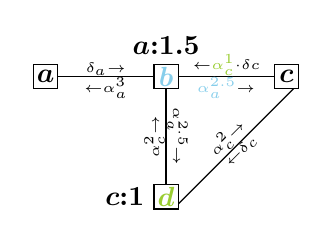
\begin{tikzpicture}[scale=0.87]

  \thickmuskip=0mu
  \medmuskip=0mu
  \thinmuskip=0mu
  
  \newcommand\X{50pt}
  \newcommand\Y{-50pt}

  \newcommand\ADD{\alpha}
  \newcommand\DEL{\delta}



  \draw (-\X + 5pt, 0) --
  node[above=-0.3em,font=\tiny]{$\DEL_{a} \rightarrow$}
  node[below=-0.3em,font=\tiny]{$\leftarrow \ADD_{a}^{3}$}
  (0 - 5pt, 0); %% b - a 

  \draw (0 +5pt, 0) --
  node[above=-0.3em, font=\tiny]{$\leftarrow \textcolor{\PC}{\ADD_{c}^{1}}\cdot\DEL{c}$}
  node[below=-0.3em, font=\tiny]{$\textcolor{\PA}{\ADD_a^{2.5}} \rightarrow$}
  (\X -5pt, 0); %% b - c

  \draw[opacity=0] (0, 0 - 5pt) --
  node[opacity=1, above=-0.3em, font=\tiny, sloped]{$\ADD_a^{2.5} \rightarrow$}
  (0, \Y + 5pt); %% b - d
  \draw (0, \Y + 5pt) --
  node[above=-0.3em, font=\tiny, sloped]{$\ADD_c^2 \rightarrow$}
  (0, 0 - 5pt);  %% d - b
  
  \draw (\X + 3pt, 0 - 5pt) --
  node[above=-0.3em, font=\tiny, sloped]{$\ADD_{c}^{2} \rightarrow$}
  node[below=-0.3em, font=\tiny, sloped]{$\leftarrow \DEL_c$}
  (0 + 5pt, \Y - 3pt); %% c - d



  
  \draw[fill=white] (-\X, 0) node{$\bm{a}$} +(-5pt, -5pt) rectangle +(5pt, 5pt);  
  \draw[fill=white] (0, 0) node[color=\PA]{$\bm{b}$} +(-5pt, -5pt) rectangle +(5pt, 5pt);
  \draw[fill=white] (\X, 0) node{$\bm{c}$} +(-5pt, -5pt) rectangle +(5pt, 5pt);
  \draw[fill=white] (0, \Y) node[color=\PC]{$\bm{d}$} +(-5pt, -5pt) rectangle +(5pt, 5pt);
  
  % \draw (-\X+5pt, 5pt) node[above left]{$\DEL_a$};
  % \draw (\X+5pt, 5pt) node[above right]{$\DEL_c$};
  \draw (0, 5pt) node[above]{$\bm{a: 1.5}$};
  \draw (-5pt, \Y) node[left]{$\bm{c: 1}$};


\end{tikzpicture}
}
  \end{center}
  \caption{\label{fig:del}Efficient removal of a partition using
    scoped broadast. $a$ eventually acknowledges that it belongs to $P_d$ with $\alpha_d^3$ echoing.}
\end{figure}

%%% Local Variables: 
%%% mode: latex
%%% TeX-master: "../paper"
%%% ispell-local-dictionary: "english"
%%% End: 



\begin{definition}[\label{def:dcp}\underline{D}ynamic
  \underline{c}onsistent \underline{p}artitioning (DCP)]
  Dynamic consistent partitioning is consistent partitioning where
  \processes can join or leave the set of sources at any \TODO{time}.
\end{definition}


A naive implementation resembles echos in acoustics:
\underline{d}elete notifications $\delta$ propagate as long as
receivers' current partition is the targeted one, and when delete
notifications reach the bordering \processes of the deleted partition,
it triggers a competition -- or an echo -- that goes backward to fill
the gap left open by removals.  For example, in Figure~\ref{fig:del},
two partitions initially exist: $P_a$ and $P_d$ that respectively
include $\{a\}$, and $\{b, c, d\}$. In Figure~\ref{fig:delA}, $a$
deletes its partition. It notifies all neighboring \processes~--~here
only $b$~-- that may belong to its partition using \NAMEB. Upon
receipt, $b$ discards the delete notification $\delta_a$ since
$\delta_a$ does not target the former's partition $P_d$. \Process~$b$
sends its own best partition $\alpha_d^3$ that may be the best for
$a$. Eventually, every \process belongs to Partition $P_d$. In this
scenario, they reach consistent partitioning.

Delete operations add a new notion of order between events, and most
importantly between message deliveries. Delete operations implicitly
state that all preceding events become obsolete, and that all messages
originating from these preceding events convey stale control
information.


\begin{definition}[Happens-before ($\rightarrow$)~\cite{lamport1978time}]
  The transitive, irreflexive, and antisymmetric happens-before
  relationship defines a strict partial order between events. Two
  messages are concurrent if none happens before the other.
\end{definition}

\begin{definition}[\label{def:lwo}Stale messages]
  Only the latest broadcast of a \node matters.  A message $m$ conveys
  \underline{s}tale control information $\mathcal{S}(m)$ as soon as
  its broadcaster broadcasts another message: $\mathcal{S}(\alpha_x) =
  \exists \delta_x: b_x(\alpha_x) \rightarrow b_x(\delta_x)$.  A
  \process only sends messages that it assumes up-to-date:
  $s_x(\alpha_s) \implies \delta_s \not\in R_x$. \TODO{Only keep last?
    Tothink what happens if we keep all as in def now.}
\end{definition}


\begin{figure*}[t]
  \newcommand{\SCALE}{0.8}

  \thickmuskip=0mu
  \medmuskip=0mu
  \thinmuskip=0mu

  \newcommand\X{42pt}
  \newcommand\Y{-40pt}

  \newcommand{\OACK}{0.5}
  \newcommand{\SMSG}{\tiny}
  
  \newcommand{\LEFT}{\triangleleft}
  \newcommand{\RIGHT}{\triangleright}
  
  \begin{center}
    \subfloat[Part A][\label{fig:undoproblemA}$a$ and $c$ become sources.
      $w_{ab} = 2$; $w_{bc} = 1$.]{
\begin{tikzpicture}[scale=\SCALE]

  %% \draw (-\X, 5pt) node[above, font=\scriptsize]{$\textcolor{\PA}{\alpha_a^0}$};
  %% \draw ( \X, 5pt) node[above, font=\scriptsize]{$\textcolor{\PC}{\alpha_c^0}\vphantom{\alpha_a^3}$};

  \begin{scope}[shift={(0, -1*\Y)}]

      \draw [opacity=0] (-1.5*\X, 0) -- (1.5*\X, 0); %% spacing
    
      \draw (-\X + 5pt, 0) --
      node[above=-0.3em,font=\SMSG]{$\textcolor{\PA}{\alpha_{a}^{2}} \RIGHT$}
      (0 - 5pt, 0); %% b - a 
      
      \draw (0 +5pt, 0) --
      node[below=-0.3em,font=\SMSG]{~ ~ ~ ~ ~$\LEFT \textcolor{\PC}{\alpha_{c}^{1}}$}
      (\X -5pt, 0); %% b - c
      
      \draw[fill=white] (-\X, 0) node{\textcolor{\PA}{$\bm{a}$}} +(-5pt, -5pt) rectangle +(5pt, 5pt);  
      \draw[fill=white] (0, 0) node{$\bm{b}$} +(-5pt, -5pt) rectangle +(5pt, 5pt);
      \draw[fill=white] (\X, 0) node{\textcolor{\PC}{$\bm{c}$}} +(-5pt, -5pt) rectangle +(5pt, 5pt);
      
      \draw (-\X, 5pt) node[above, font=\scriptsize]{$\textcolor{\PA}{\alpha_a^0}$};
      \draw ( \X, 5pt) node[above, font=\scriptsize]{$\textcolor{\PC}{\alpha_c^0}\vphantom{\alpha_a^3}$};
    
  \end{scope}
  
\end{tikzpicture}
}
    \hspace{5pt}
    \subfloat[Part B][\label{fig:undoproblemB}$c$ deletes its partition but $a$ does not.
      $b$ delivers and forwards $\alpha_a$.]
             {

\begin{tikzpicture}[scale=\SCALE]

  \thickmuskip=0mu
  \medmuskip=0mu
  \thinmuskip=0mu
  
  \newcommand\X{50pt}
  \newcommand\Y{-50pt}

  \newcommand\ADD{\alpha}
  \newcommand\DEL{\delta}


  
%%   \draw (-\X + 5pt, 0) --
%%   node[above=-0.3em,font=\tiny]{$\bm{\DEL_{a} \RIGHT}$}
%%   (0 - 5pt, 0); %% b - a 

%%   \draw (0 +5pt, 0) --
%%   node[above=-0.3em,font=\tiny]{$\textcolor{\PA}{\ADD_{a}^{3}} \RIGHT$}
%%   node[below=-0.3em,font=\tiny]{$\LEFT \textcolor{\PC}{\ADD_{c}^{1}} \cdot \DEL_c$}
%%   (\X -5pt, 0); %% b - c

%% 
  
%%   \draw[fill=white] (-\X, 0) node{$\bm{a}$} +(-5pt, -5pt) rectangle +(5pt, 5pt);  
%%   \draw[fill=white] (0, 0) node{\textcolor{\PA}{$\bm{b}$}} +(-5pt, -5pt) rectangle +(5pt, 5pt);
%%   \draw[fill=white] (\X, 0) node{$\bm{c}$} +(-5pt, -5pt) rectangle +(5pt, 5pt);
  
%%   \draw (-\X, 5pt) node[above, font=\scriptsize]{$\textcolor{\PA}{\ADD_a} \bm{\rightarrow \DEL_a}$};
%%   \draw (  0, 5pt) node[above, font=\scriptsize]{$\textcolor{\PA}{\ADD_a^2}$};
%%   \draw ( \X, 5pt) node[above, font=\scriptsize]{$\textcolor{\PC}{\ADD_c}\vphantom{\ADD_a^3} \rightarrow \DEL_c$};

  \begin{scope}[shift={(0, -1*\Y)}]
      \draw (-\X + 5pt, 0) --
      (0 - 5pt, 0); %% b - a 
      
      \draw (0 +5pt, 0) --
      node[above=-0.3em,font=\tiny]{$\textcolor{\PA}{\ADD_{a}^{3}} \RIGHT$}
      node[below=-0.3em,font=\tiny]{$\LEFT \textcolor{\PC}{\ADD_{c}^{1}} \cdot \DEL_c$}
      (\X -5pt, 0); %% b - c
      
      \draw[fill=white] (-\X, 0) node{\textcolor{\PA}{$\bm{a}$}} +(-5pt, -5pt) rectangle +(5pt, 5pt);  
      \draw[fill=white] (0, 0) node{\textcolor{\PA}{$\bm{b}$}} +(-5pt, -5pt) rectangle +(5pt, 5pt);
      \draw[fill=white] (\X, 0) node{$\bm{c}$} +(-5pt, -5pt) rectangle +(5pt, 5pt);
      
      \draw (-\X, 5pt) node[above, font=\scriptsize]{$\textcolor{\PA}{\ADD_a^0}$};
      \draw (  0, 5pt) node[above, font=\scriptsize]{$\textcolor{\PA}{\ADD_a^2}$};
      \draw ( \X, 5pt) node[above, font=\scriptsize]{$\textcolor{\PC}{\ADD_c}\vphantom{\ADD_a^3} \rightarrow \DEL_c$};

  \end{scope}

\end{tikzpicture}
}
    \hspace{5pt}
    \subfloat[Part C][\label{fig:undoproblemC}$b$ delivers + forwards $\alpha_c$.]
             {
\begin{tikzpicture}[scale=\SCALE]

    \draw [opacity=0] (-1.5*\X, 0) -- (1.5*\X, 0); %% spacing
    
    \draw (-\X + 5pt, 0) --
    node[below=-0.3em, font=\SMSG]{$\LEFT \textcolor{\PC}{\alpha_c^3}$} %% b - a
    (0 - 5pt, 0);
    
    \draw [<->] (0 +5pt, 0) --
    node[opacity=\OACK, above=-0.3em, font=\SMSG]{$\alpha_c^2 \RIGHT$~ ~ ~}
    node[below=-0.3em, font=\SMSG]{$\LEFT \delta_c \vphantom{\alpha^1}$~ ~ ~ }
    node[opacity=\OACK, below=-0.3em, font=\SMSG]{~ ~ ~ $\LEFT \alpha_a^4$}
    (\X -5pt, 0); %% b - c
    
    \draw[fill=white] (-\X, 0) node{\textcolor{\PA}{$\bm{a}$}} +(-5pt, -5pt) rectangle +(5pt, 5pt);  
    \draw[fill=white] (0, 0) node{\textcolor{\PC}{$\bm{b}$}} +(-5pt, -5pt) rectangle +(5pt, 5pt);
    \draw[fill=white] (\X, 0) node{\textcolor{\PA}{$\bm{c}$}} +(-5pt, -5pt) rectangle +(5pt, 5pt);
    
    \draw (-\X, -6pt) node[below, font=\SNODE]{$\textcolor{\PA}{\alpha_a^0}$};
    \draw (  0,  6pt) node[above, font=\SNODE]{$\textcolor{\PA}{\alpha_a^2} \rightarrow \textcolor{\PC}{\alpha_c^1}$};
    \draw ( \X, -6pt) node[below, font=\SNODE]{$\textcolor{\PC}{\alpha_c}\vphantom{\alpha_a^3} \rightarrow \delta_c \rightarrow \textcolor{\PA}{\alpha_a^3}$};
    

\end{tikzpicture}
}
    \hspace{5pt}
    \subfloat[Part D][\label{fig:undoproblemD}$b$ delivers + forwards $\delta_c$.]
             {
\begin{tikzpicture}[scale=\SCALE]

  \thickmuskip=0mu
  \medmuskip=0mu
  \thinmuskip=0mu
  
  \newcommand\X{50pt}
  \newcommand\Y{-50pt}

  \newcommand\ADD{\alpha}
  \newcommand\DEL{\delta}


  
%%   \draw (-\X + 5pt, 0) --
%%   (0 - 5pt, 0);

%%   \draw (0 +5pt, 0) --
%%   node[below=-0.3em, font=\tiny]{$\vphantom{\ADD^1_c }$}
%%   (\X -5pt, 0); %% b - c

%% 
  
%%   \draw[fill=white] (-\X, 0) node{$\bm{a}$} +(-5pt, -5pt) rectangle +(5pt, 5pt);  
%%   \draw[fill=white] (0, 0) node{$\bm{b}$} +(-5pt, -5pt) rectangle +(5pt, 5pt);
%%   \draw[color=\WRONG, fill=white] (\X, 0) node{\textcolor{\PA}{$\bm{c}$}} +(-5pt, -5pt) rectangle +(5pt, 5pt);
  
%%   \draw (-\X, 5pt) node[above, font=\scriptsize]{$\ldots \rightarrow \textcolor{\PC}{\ADD_c} \rightarrow \DEL_c$};
%%   \draw (  0, 5pt) node[above, font=\scriptsize]{$\ldots \rightarrow \DEL_c$};
%%   \draw ( \X, 5pt) node[above, font=\scriptsize]{$\ldots \rightarrow \textcolor{\PA}{\ADD_a^3}$};


  
  \begin{scope}[shift={(0, -1*\Y)}]

    \draw (-\X + 5pt, 0) --
    (0 - 5pt, 0);
    
    \draw (0 +5pt, 0) --
    node[below=-0.3em, font=\tiny]{$\vphantom{\ADD^1_c }$}
    (\X -5pt, 0); %% b - c

    
    \draw[fill=white] (-\X, 0) node{\textcolor{\PA}{$\bm{a}$}} +(-5pt, -5pt) rectangle +(5pt, 5pt);  
    \draw[fill=white] (0, 0) node{\textcolor{\PA}{$\bm{b}$}} +(-5pt, -5pt) rectangle +(5pt, 5pt);
    \draw[fill=white] (\X, 0) node{\textcolor{\PA}{$\bm{c}$}} +(-5pt, -5pt) rectangle +(5pt, 5pt);
    
    \draw (-\X, 5pt) node[above, font=\scriptsize]{$\textcolor{\PA}{\ADD_a^0}$};
    \draw (  0, 5pt) node[above, font=\scriptsize]{$\ldots \rightarrow \DEL_c \rightarrow \textcolor{\PA}{\ADD_a^2}$};
    \draw ( \X, 5pt) node[above, font=\scriptsize]{$\ldots \rightarrow \textcolor{\PA}{\ADD_a^3}$};
  \end{scope}
  
\end{tikzpicture}
}
    \hspace{5pt}
    \subfloat[Part E][\label{fig:undoproblemE}$a$ echoes back $\alpha_a^2$ to $b$.]
             {
\begin{tikzpicture}[scale=\SCALE]

%%   \draw (-\X + 5pt, 0) --
%%   node[above=-0.3em, font=\tiny]{~ ~ ~ ~ ~ $\delta_{a} \RIGHT$} %% b - a
%%   node[above=-0.3em, font=\tiny]{~ ~ ~ ~ ~ $\textcolor{\WRONG}{\text{\normalsize\xmark}} \hphantom{\RIGHT}$} %% b - a
%%   node[below=-0.3em, font=\tiny]{$\LEFT \textcolor{\PC}{\alpha_c^3}$} %% b - a
%%   (0 - 5pt, 0);

%%   \draw (0 +5pt, 0) --
%%   node[below=-0.3em, font=\tiny]{$\LEFT \delta_c \vphantom{\alpha^1}$}
%%   (\X -5pt, 0); %% b - c

%% 
  
%%   \draw[fill=white] (-\X, 0) node{$\bm{a}$} +(-5pt, -5pt) rectangle +(5pt, 5pt);  
%%   \draw[fill=white] (0, 0) node{\textcolor{\PC}{$\bm{b}$}} +(-5pt, -5pt) rectangle +(5pt, 5pt);
%%   \draw[fill=white] (\X, 0) node{\textcolor{\PA}{$\bm{c}$}} +(-5pt, -5pt) rectangle +(5pt, 5pt);
  
%%   \draw (-\X, 5pt) node[above, font=\scriptsize]{$\textcolor{\PA}{\alpha_a}\rightarrow \delta_a$};
%%   \draw (  0, 5pt) node[above, font=\scriptsize]{$\textcolor{\PA}{\alpha_a^2} \rightarrow \textcolor{\PC}{\alpha_c^1}$};
%%   \draw ( \X, 5pt) node[above, font=\scriptsize]{$\textcolor{\PC}{\alpha_c}\vphantom{\alpha_a^3} \rightarrow \delta_c \rightarrow \textcolor{\PA}{\alpha_a^3}$};


  \begin{scope}[shift={(0, -1*\Y)}]

    \draw [opacity=0] (-1.5*\X, 0) -- (1.5*\X, 0); %% spacing

    
    \draw (-\X + 5pt, 0) --
    node[above=-0.3em, font=\SMSG]{$\textcolor{\PA}{\alpha_a^2} \RIGHT$} %% b - a
    (0 - 5pt, 0);
    
    \draw [<->] (0 +5pt, 0) --
    node[opacity=\OACK, above=-0.3em, font=\SMSG]{~ ~ ~ ~ ~ ~$\alpha_c^2 \RIGHT$}
    node[opacity=\OACK, below=-0.3em, font=\SMSG]{$\LEFT \alpha_a^4$~ ~ ~ ~ ~ ~}
    (\X -5pt, 0); %% b - c
    
    \draw[fill=white] (-\X, 0) node{\textcolor{\PA}{$\bm{a}$}} +(-5pt, -5pt) rectangle +(5pt, 5pt);  
    \draw[fill=white] (0, 0) node{$\bm{b}$} +(-5pt, -5pt) rectangle +(5pt, 5pt);
    \draw[fill=white] (\X, 0) node{\textcolor{\PA}{$\bm{c}$}} +(-5pt, -5pt) rectangle +(5pt, 5pt);
    
    \draw (-\X, 5pt) node[above, font=\scriptsize]{$\textcolor{\PA}{\alpha_a^0}$};
    \draw (  0, 5pt) node[above, font=\scriptsize]{$\ldots \rightarrow \delta_c$};
    \draw ( \X, 5pt) node[above, font=\scriptsize]{$\textcolor{\PC}{\alpha_c}\vphantom{\alpha_a^3} \rightarrow \delta_c \rightarrow \textcolor{\PA}{\alpha_a^3}$};
    
  \end{scope}

\end{tikzpicture}
}
    \hspace{5pt}
    \subfloat[Part F][\label{fig:undoproblemF}$a$, $b$, $c$ belong to $P_a$.]
             {
\begin{tikzpicture}[scale=\SCALE]


  
  \draw [opacity=0] (-1.5*\X, 0) -- (1.5*\X, 0); %% spacing
  
  \draw [->](-\X + 5pt, 0) --
  node[opacity=\OACK, below=-0.3em, font=\SMSG]{$\LEFT \alpha_a^4$} 
  (0 - 5pt, 0);
  
  \draw [->] (0 +5pt, 0) --
  node[above=-0.3em, font=\SMSG]{$\textcolor{\PA}{\alpha^3_a} \RIGHT$}
  (\X -5pt, 0); %% b - c
  
  
  \draw[fill=white] (-\X, 0) node{\textcolor{\PA}{$\bm{a}$}} +(-5pt, -5pt) rectangle +(5pt, 5pt);  
  \draw[fill=white] (0, 0) node{\textcolor{\PA}{$\bm{b}$}} +(-5pt, -5pt) rectangle +(5pt, 5pt);
  \draw[fill=white] (\X, 0) node{\textcolor{\PA}{$\bm{c}$}} +(-5pt, -5pt) rectangle +(5pt, 5pt);
  
  \draw (-\X, -6pt) node[below, font=\SNODE]{$\textcolor{\PA}{\alpha_a^0}$};
  \draw (  0,  6pt) node[above, font=\SNODE]{$\ldots \rightarrow \textcolor{\PA}{\alpha_a^2}$};
  \draw ( \X, -6pt) node[below, font=\SNODE]{$\ldots \rightarrow \textcolor{\PA}{\alpha_a^3}$};

  
\end{tikzpicture}
}
  \end{center}
  \caption{\label{fig:undoproblem}From $c$'s perspective,
    Figure~\ref{fig:problemE} and Figure~\ref{fig:undoproblemE} are
    similar in terms of received messages, but the outcomes eventually
    differ. Yet, $c$ must act on Figure~\ref{fig:undoproblemE}, and
    acknowledge then propagate the \emph{possible} staleness of
    Partition $P_a$.}
\end{figure*}



\begin{definition}[\label{def:fs}\underline{F}orwarding of
    \underline{s}taleness (FS)]
  %
  To \NAMEB staleness, a \process $x$ delivers and forwards a received
  staleness notification if it is not yet delivered and targets its
  best delivered message: $\delta_s \in R_x \setminus D_x \wedge
  \alpha_s = \min D_x \TODO{\implies} d_x(\delta_s) \wedge
  f_x(\delta_s)$.
\end{definition}

\begin{definition}[\label{def:fbplus}FB$^+$: echos] FB where a
  \process $x$ that receives a staleness notification sends back --~or
  echoes~-- its best up-to-date delivered message: $r_{xy}(\alpha_s)
  \wedge \delta_s \in D_x \implies s_{xy}(\alpha_{s'})$ with
  $\alpha_{s'} = \min D_x \wedge \delta_{s'} \not\in
  D_x$. \TODO{Rework min}
\end{definition}

\TODO{Naive implementation is FB$^+$ etc. It does not work.}

\begin{lemma}[\label{lem:fbfse}FB$^+ \wedge$ FS $\centernot\implies$ DCP]
  Forwarding best up-to-date, forwarding staleness, and echoing is not
  sufficient to guarantee dynamic consistent partitioning.
\end{lemma}

\begin{proof}
Stale control information as stated in Definition~\ref{def:lwo} may
impair the propagation of both
\begin{inparaenum}[(i)]
\item notifications about actual sources, and
\item notifications about deleted partitions.
\end{inparaenum}
Figure~\ref{fig:problem} depicts a scenario comprising only three
\processes $a$, $b$, $c$ chained with FIFO links, \ie where \processes
receive the messages in the order of their sending ($s_{pq}(m)
\rightarrow s_{pq}(m') \implies r_q(m) \rightarrow r_q(m')$). In
Figure~\ref{fig:problemA}, both $a$ and $c$ become sources, sending
their respective notification message to $b$. In
Figure~\ref{fig:problemB}, both $a$ and $c$ delete their partition
while $b$ receives, delivers, and forwards $\alpha_a^2$. In
Figure~\ref{fig:problemC}, $b$ receives, delivers, and forwards
$\alpha_c^1$, for it improves its best partition. Then it receives and
discards $\delta_a$, for its best partition does not match the deleted
one. We simplify the echo since $\alpha_c^3$ is already transiting
towards $a$. Finally, Figure~\ref{fig:problemD} shows that eventually,
$c$ stays in the deleted partition $P_a$ for not having received
$\delta_a$ that $b$ blocked earlier. The system does not reach
consistent partitioning. \end{proof}

As a cascading effect, in Figure~\ref{fig:problemD}, not only $c$
wrongfully believes that it belongs to $a$'s partition when $a$
already deleted it, but it could contribute to its inconsistency by
blocking farther but up-to-date messages from actual sources. To reach
consistent partitioning, \processes need
\begin{inparaenum}[(i)]
\item to detect possibly blocking conditions 
\item to purge all stale messages from the system
\item enabling up-to-date notifications to eventually echo back to
  every \process.
\end{inparaenum}

\begin{lemma}[\label{lem:detector}$\textup{FB}^+ \wedge \textup{FS}
  \implies$ \underline{D}etector existence (D)] Assuming
  $\textup{FB}^+$, $\textup{FS}$, a chain of delivery on $\pi_{xz}$ of
  $\alpha_x$ with $\alpha_x = \min D_z$, if $x$ broadcasts a staleness
  notification $\delta_x$, either $z$ eventually delivers it, or a
  \process $y$ in such a chain of delivery $\pi_{xz}'$ eventually
  \TODO{detects} its \TODO{blocking}.
  % $b_p(\delta_x) \implies d_q(x) U Detect[X]$ ??? 
\end{lemma}


\begin{proof}
  %% knowing that b_p delta is sufficient to say that processes will
  %% receive delta or detect blocking
  (A) Assuming a chain of delivery $\pi_{xz} = [x, \ldots, z]$ of
  $\alpha_x$ with $\forall y \in \pi_{xz}: \alpha_x = \min D_y$, and
  assuming $d_x(\delta_x)$, then with forwarding of staleness
  (Definition~\ref{def:fs}),
  $f_{\pi_{xz}[k]}(\delta_x) \implies \eventually
  d_{\pi_{xz}[k+1]}(\delta_x)$ except if $\delta_x \in D_{\pi_{xz}[k+1]}$ which
  means that $\pi_{xz}[k+1]$ already delivered and forwarded $\delta_x$
  following another such a chain of delivery. Therefore, $z$
  eventually receives, hence delivers $\delta_x$.

  \noindent (B) Assuming a chain of delivery
  $\pi_{xz} = [x, \ldots, z]$ of $\alpha_x$ with at least
  $\alpha_x = \min D_z$, and assuming $d_x(\delta_x)$, then by (A),
  the staleness notification reaches a \process $ y = \pi_{xz}[k]$. By
  Definition~\ref{def:fs}, the forwarding stops when $y$ already
  delivered $\delta_x$ ($\delta_x \in D_y$ covered by (A)) or
  delivered a better message $\alpha_s = \min D_y$ with
  $\alpha_s \neq \alpha_x$. With $y'=\pi_{xz}[k+1]$, forwarding of
  best (Definition~\ref{def:fbplus}) implies three possible outcomes:
  \begin{enumerate}[(i)]
  \item $\alpha_{s'} = \min D_{y'}$ with $\alpha_{s'} \neq \alpha_x$
    hence $y' \iff y$ which leaves two possible outcomes:
  \item
    $r_{y'}(\alpha_s) \wedge \alpha_x = \min D_{y'} \wedge \alpha_x <
    \alpha_s$ which means that a shorter path of delivery $\pi_{xz}'$
    exists that either forwards appropriate staleness notifications
    (A) or detects its possible blocking:
  \item
    $r_{y'}(\alpha_s) \wedge \delta_s \in D_{y'} \wedge \alpha_x =
    \min D_{y'}$ which detects a possible blocking of
    $\delta_x$. Without global knowledge, $y'$ assumes it belongs to
    the shortest and only path of delivery of $\alpha_x$
    ($\pi_{xy'} \subseteq \Pi_{xz}$) thus it does not further delegate
    the detection to another \process.
  \end{enumerate} \vspace{-1.5em} %% ugly vspace but necessary for enumerate+qed
  %
  %% (i) If every \process (such as $a$) starting from the source
  %% delivers and forwards a removal notification $\delta_X$ when their
  %% last delivery is $\alpha_X$, then every such \process eventually
  %% delivers the removal notification $\delta_X$ except \processes (such
  %% as $b$) that delivered $\alpha_X$ from a \process that delivered a
  %% message from another partition $\alpha_Y$ since then.
  %
  %% These exceptions eventually receive and deliver $\alpha_Y$ since
  %% $\alpha_Y$ is better than $\alpha_X$ through this path, except if
  %% they already received and delivered the removal notification of
  %% $P_Y$ (such as $c$). These \processes may never receive hence
  %% deliver $\delta_X$, and may never receive hence deliver a better
  %% message than $\alpha_X$. They need an additional mechanism to
  %% eventually purge $\alpha_X$ that cannot rely on the eventual purging
  %% of $P_Y$ at \processes like $b$, to avoid deadlocks.
  %
  %% (ii) Assuming that every \process keeps an history of its past
  %% deliveries, \processes (such as $c$) can detect the inconsistency,
  %% since they receive from their parent an already deleted partition
  %% $P_Y$. This notification means that the parent discards any
  %% $\delta_Z$ with $\alpha_Z^z < \alpha_Y^y$, and most importantly, if
  %% $\delta_X$ exists, it discards it. To ensure the purge of stale
  %% messages, a detecting \process must assume the worst case that such
  %% $\delta_X$ exists, and send another kind of message, noted $\Delta$,
  %% that notify the possible removal of $P_X$.
  %
  %% (iii) A \process (such as $d$) whose last delivery is $\alpha_X$,
  %% but whose parent is neither inconsistent (like $b$) nor receiving
  %% $\delta_X$ (like $a$), eventually receives $\Delta$ from a detecting
  %% \process, either directly or transitively, for such a child \process
  %% ($d$) trusts the possible removal of $P_X$ by delivering and
  %% forwarding such $\Delta$. $\Delta$ suffers from identical blocking
  %% conditions (between $b$ and $c$) than $\delta$, leading to the same
  %% solutions of detection and propagation of $\Delta$. Eventually,
  %% every \process whose last delivery is $\alpha_X$ receives and
  %% delivers either a better $\alpha_Z$, or $\delta_X$, or $\Delta_X$.
\end{proof}

Proof of Lemma~\ref{lem:detector} shows that there exists false
positive in the blocking detection: $\delta_x$ may not exist but $y'$
still receives $\alpha_s$ after the delivery of $\delta_s$ from the
path it delivered $\alpha_x$. Figure~\ref{fig:undoproblem} highlights
this behavior. In Figure~\ref{fig:undoproblemB}, $a$ does not delete
its partition. In Figure~\ref{fig:undoproblemD} and because of \NAMEB,
$c$ received the same series of messages as in
Figure~\ref{fig:problemD}. Yet, $c$ must assume the existence of
$\delta_a$ and act accordingly by forcing the staleness of its best
delivered message and disseminate this information to its neighbors.
To avoid flooding the system with false positive staleness
notifications, we propose to reduce the scope of staleness
notifications by including only downstream \processes. In
Figure~\ref{fig:undoproblemD}, false positives would not affect $a$
and $b$.

\begin{definition}[\label{def:fsplus}$\textup{FS}^+$: forwarding
  staleness downstream]
  To \NAMEB staleness downstream, a node $x$ delivers and forwards a
  received staleness notification if it is not yet delivered and it
  comes from the path of delivery of its best up-to-date delivered
  message. \TODO{more.}
\end{definition}

It is worth noting that forwarding of staleness as stated in
Definition~\ref{def:fs} becomes a specific case of
Definition~\ref{def:fsplus} where the source itself forwards a
staleness notification downstream. The notification must reach all
\processes in its partition since the source has no \processes
upstream, and belongs to the delivery path of all \processes that
delivered this message.

\TODO{$FB \subseteq FB+$}.

\begin{theorem}[$\textup{FB}^+ \wedge \textup{FS}^+ \TODO{\wedge \textup{D}} \implies \textup{DCP}$]
  A protocol guarantees dynamic consistent partitioning if it
  implements forwarding of best up-to-date messages with echos,
  forwarding of staleness messages downstream, and detection of
  possible blocking of staleness notifications.
\end{theorem}

\begin{proof}
  Detection triggers forwarding of staleness downstream which
  completes the case study of Lemma~\ref{lem:detector} by ensuring
  that, when a source broadcasts its staleness notification, all
  \processes that belong to its partition eventually deliver such a
  staleness notification. All downstream bordering \processes also
  eventually receive such a staleness notification and echo back their
  best delivered message. This triggers another competition as in
  Theorem~\ref{theo:fb} for the \processes that delivered the
  staleness notification.
\end{proof}

\begin{algorithm}
  
\SetInd{0.2em}{0.8em}

\newcommand{\algoAnd}{~\textbf{\textup{and}}~}
\newcommand{\algoOr}{~\textbf{\textup{or}}~}

\SetKwProg{Function}{func}{}{}

\small

\DontPrintSemicolon
\LinesNumbered

$O_p$, $W_p$ \tcp*[r]{set of neighbors and weights}
$A_{s, c}^{d, \pi} \leftarrow \alpha_{\infty, 0}^{\infty, \varnothing} $ \tcp*[r]{best $\alpha$ so far}
$V \leftarrow \varnothing$;~ $V[p] \leftarrow 0$ \tcp*[r]{vector of versions}

\BlankLine
\BlankLine

\begin{multicols}{2}
\Function{\textup{\texttt{Add ( )}}} { % \hfill [if $V[p]\equiv 0 \mod 2 $]} } {
  \textup{\smash{receiveAdd($p$, $\alpha_{p, V[p] + 1}^{0, \varnothing}$)}}\label{line:ascast_add}
}

% \BlankLine

\Function{\textup{\texttt{Del ( )}}} { % \hfill [if $V[p]\equiv 1 \mod 2 $]} } {
  \textup{\smash{receiveDel($p$, $\delta_{p, V[p] + 1}$)}}\label{line:ascast_del}
}
\end{multicols}

\BlankLine
\BlankLine
\BlankLine

\begin{multicols}{2}
\Function{\textup{receiveAdd($q$, $\alpha_{s', c'}^{d', \pi'}$)}}
  %\tcp*[f]{\footnotesize{receive $\alpha$ from $q$}}}
  {
    \uIf{\hphantom{$($}$q = \pi[|\pi| - 1] \algoAnd$\tcp*[h]{{\footnotesize{from parent?}}}\\
    \hphantom{\textbf{if}} $(c' < V[s'] \,\, \algoOr$\tcp*[h]{\footnotesize{history or state?}\label{line:ascast_version}}\\
    \hphantom{\textbf{if}} \smash{$(\alpha_{s', c'}^{d', \pi'} > A_{s, c}^{d, \pi} \algoAnd  p\not\in \pi'))$}\label{line:detectA}} {
        \textup{receiveDel($q$, $\delta_{s, c}^{\pi}$)} \tcp*[h]{\footnotesize{(II) send $\Delta$}}
    }
    \uElseIf {$A_{s, c}^{d, \pi} < \alpha_{s', c'}^{d', \pi} \algoAnd p \not\in \pi'$  } {
          $V[s'] \leftarrow c'$ \;
          $\smash{A_{s, c}^{d, \pi} \leftarrow \alpha_{s', c'}^{d', \pi'}}$ \;
          \ForEach{$n \in O_p$} {
            send$_n$(\smash{$\alpha_{s', c'}^{d' + W_{pq}, \pi' \cup p}$)} \tcp*[h]{\footnotesize{forward}\label{line:ascast_better}}
          }

     }
}



\Function{\textup{receiveDel($q$, $\delta_{s', c'}^{\pi'}$)}
%  \tcp*[f]{\footnotesize \smash{$r_p (\delta_{s', c'})$ \textup{\texttt{or}} $r_p (\delta_{s', c'}^{\pi'})$}}
} {
  \uIf(\tcp*[h]{\hspace{-0.5em}\footnotesize{$\Delta$?}}){\hphantom{$(($}$p \not\in \pi'$ \algoAnd \label{line:notloopingB}\tcp*[h]{\footnotesize{looping?}}\\
    \hphantom{\textbf{if} }$((\delta_{s', c'} \algoAnd \alpha_{s', c'-1} = A_{s, c})  \algoOr$\tcp*[h]{$\delta$?}\\
    \hphantom{\textbf{if} }\smash{$(\delta_{s',c'}^{\pi'}  \algoAnd  \alpha_{s', c'}^{\_, \pi'} = A_{s, c}^{\_, \pi}))$}} {
     $V[s'] \leftarrow \max(V[s'], c')$ \;
     $A_{s, c}^{d, \pi} \leftarrow \alpha_{\infty, 0}^{\infty, \varnothing}$ \;

    \ForEach{$n \in O_p$}{
      \lIf(\tcp*[h]{\footnotesize{(I)}}) {\smash{$\delta_{s', c'}$}} {
        send$_n$(\smash{$\delta_{s', c'}$)}
      } 
      \hphantom{\textbf{if} $\delta_{s', c'}^{\pi'}$}~\textbf{else} send$_n$(\smash{$\delta_{s', c'}^{\pi'\cup p}$)}~\tcp*[h]{\footnotesize{(III)}}
    }

  }\uElseIf{$A_{s, c}^{d, \pi} \neq \alpha_{\infty, 0}^{\infty, \varnothing}$} {
     \textup{send$_q$($\alpha_{s, c}^{d + W_{pq}, \pi \cup p}$)}
     \tcp*[h]{\label{line:ascast_compete}\footnotesize{compete again}}
  }
}

\end{multicols}

\BlankLine
\BlankLine
\BlankLine

%% \Function{\textup{edgeUp($q$)} \tcp*[f]{new link to $q$}}  {
%%     \If {$A_{s, c}^{d, \pi} \neq \alpha_{\infty, 0}^{\infty, \varnothing}$} {
%%          \textup{send$_q$($\alpha_{s, c}^{d + W_{pq}, \pi \cup p}$)}
%%          \tcp*[r]{\label{line:compete}\footnotesize{compete with $q$}}}
%% }

%% \BlankLine

%% \Function{\textup{edgeDown($q$)} \tcp*[f]{link to $q$ removed}} {
%%   \If {$q = \pi[|\pi| - 1]$} {
%%     \textup{receiveDel($q$, $\delta_{s, c}^{\pi}$)} \tcp*[r]{\footnotesize IV: $\delta?$ propagation}
%%   }
%% }

\begin{multicols}{2}
\Function{\textup{edgeUp($q$)} \tcp*[h]{new link to $q$}}  {
    \If {$A_{s, c}^{d, \pi} \neq \alpha_{\infty, 0}^{\infty, \varnothing}$} {
         \textup{send$_q$($\alpha_{s, c}^{d + W_{pq}, \pi \cup p}$)}
         \tcp*[h]{\label{line:compete}\footnotesize{compete with $q$}}}
}

% \BlankLine

\Function{\textup{edgeDown($q$)} \tcp*[h]{link to $q$ removed}} {
  \If {$q = \pi[|\pi| - 1]$} {
    \textup{receiveDel($q$, $\delta_{s, c}^{\pi}$)} \tcp*[h]{\footnotesize (III) send $\Delta$}
  }
}

\end{multicols}

\BlankLine

%%% Local Variables: 
%%% mode: latex
%%% TeX-master: "../paper"
%%% ispell-local-dictionary: "english"
%%% End: 

  \caption{\label{algo:ascast}\NAME at \Process~$p$.}
\end{algorithm}

Algorithm~\ref{algo:ascast} shows the instructions of our
implementation called \NAME that enables dynamic consistent
partitioning. It implements forwarding of best (see
Line~\ref{line:fb}) and echos (see Line~\ref{line:echo}). To implement
forwarding of staleness downstream as stated in
Definition~\ref{def:fsplus},
\begin{inparaenum}[(A)]
\item each \process maintains a vector of versions that associates the
  respective known local counter of each known source, or has-been
  source. It constitutes a summary of known progress of other
  \processes; 
\item each notification message $\alpha$ carries the list of
  identifier and counter of each \node that forwarded it. In the worst
  case, both these structures grow linearly with the number of
  \processes in the system $\mathcal{O}(V)$. Nevertheless, following
  the principles of scoped broadcast, we expect that \processes only
  acknowledge a small subset of sources and messages;
\item each staleness notifications $\delta$ only carry the identifier
  and counter of the \process~--~source or detector~--~that generated
  it. Only downstream \processes may deliver such message, since they
  carry the identifier of the generator. 
\end{inparaenum}
To implement the detection as stated in Lemma~\ref{lem:detector}, each
\process only requires to know the direct parent of its best delivered
message which is already included in the piggybacked path of this
message. Receiving a message known to be stale from this parent
triggers the generation of staleness notifications that force
downstream \processes to reevaluate the partition they are in (see
Line~\ref{line:detect}).

\begin{algorithm}[h]
  \SetKwProg{Function}{func}{}{}

\SetInd{0.2em}{1em}

\small

\DontPrintSemicolon
\LinesNumbered

% \begin{multicols}{2}
\Function(\tcp*[f]{new link to $q$}){\textup{edgeUp($q$)}}  {
    \lIf {$A_{\pi}^{d} \neq \alpha_\varnothing^\infty$} {
         send$_q$($\alpha_{\pi}^{d + W_{pq}}$)
         }
}

% \BlankLine

\Function(\tcp*[f]{link to $q$ removed}){\textup{edgeDown($q$)}} {
  \lIf {\textup{isParent($q$)}} {
       receiveDel($q$, $\delta_{p, V[p]+1}$)
  }
}

% \end{multicols}

% \BlankLine

  \caption{\label{algo:edges}\NAME at \Process~$p$ in dynamic networks.}
\end{algorithm}

By reusing \NAME's default behavior, Algorithm~\ref{algo:edges}
enables dynamic consistent partitioning in dynamic networks where
\processes can join, leave, or crash at any time.  Adding a \process
is equivalent to add as many edges as necessary. Since adding an edge
may improve shortest paths, the protocol triggers a competition using
echos of Definition~\ref{def:fbplus}.  Removing a \process is
equivalent to removing all its edges. Removing an edge between two
\processes may invalidate the shortest path of one of involved
\processes plus downstream \processes, or impair the propagation of
staleness notifications. Therefore, the protocol reuses its detection
mechanism of Lemma~\ref{lem:detector} as a solution.
Algorithm~\ref{algo:edges} even extends \NAME to dynamic networks
subject to physical partitioning.

%% \NAME guarantees dynamic consistent partitioning by making extensive
%% use of \process-to-\process communications. It requires
%% \begin{inparaenum}[(i)]
%% \item purging stale control information, hence propagating $\delta$
%%   messages; and
%% \item retrieving the closest source, hence propagating $\alpha$
%%   messages.
%% \end{inparaenum}
\TODO{TODOUBLECHECK}. In terms of number of messages, in the average
case, a \process $i$ chosen uniformly at random among all \processes
creates a logical partition. Its messages $\alpha_i$ spread through
the network until reaching \processes that belong to another partition
closer to them. This splits partitions in half on average. Overall,
the $a^{th}$ new partition comprises
\smash{$\mathcal{O}(\frac{|V|}{2^{\lfloor \log_2 a \rfloor}})$}
\processes. This decreases every new partition until reaching one
\process per new partition: its source. The average number of messages
per \process is \smash{$\mathcal{O}(\frac{\overline{|O|}}{2^{\lfloor
      \log_2 a \rfloor}})$}, where \smash{$\overline{|O|}$} is the
average number of neighbors per \process.
% \TODO{Multiple receipt and
% multiple
%  delivery imply more messages (receipt bounded by $|O|$ as well).}
Deleting the $a^{th}$ partition generates twice as many messages as
creating the $a^{th}$ partition: $\delta$ messages travel through the
partition, then $\alpha$ messages compete to fill the gap.  Overall,
the communication complexity shows that \NAME scales well to the
number of partitions.
%% In the
%% worst-case, every new partition includes all but one \process
%% belonging to the previous partition. The total number of messages
%% after the $a^{th}$ new partition is $\mathcal{O}(\overline{|O|}\cdot
%% a^2)$. As for the average-case, the number of messages for the
%% partition deletion is identical to the number of messages of the
%% corresponding partition creation.
%% \begin{algorithm}[h!]
%%   \SetKwProg{Function}{func}{}{}

\SetInd{0.2em}{1em}

\small

\DontPrintSemicolon
\LinesNumbered

% \begin{multicols}{2}
\Function(\tcp*[f]{new link to $q$}){\textup{edgeUp($q$)}}  {
    \lIf {$A_{\pi}^{d} \neq \alpha_\varnothing^\infty$} {
         send$_q$($\alpha_{\pi}^{d + W_{pq}}$)
         }
}

% \BlankLine

\Function(\tcp*[f]{link to $q$ removed}){\textup{edgeDown($q$)}} {
  \lIf {\textup{isParent($q$)}} {
       receiveDel($q$, $\delta_{p, V[p]+1}$)
  }
}

% \end{multicols}

% \BlankLine

%%   \caption{\label{algo:edges}\NAME at \Process~$p$ in dynamic networks.}
%% \end{algorithm}





\subsection{Lazy dynamic consistent partitioning}
\label{subsec:lazy}

In Edge infrastructures comprising tens of thousands of autonomous
systems~\cite{nur2018crossas}, only a small subset of autonomous
systems needs logical partitioning. At any time, an autonomous system
start logical partitioning when a \process from this network becomes a
source.  Then every \process from this network belongs to the
partition of its closest source not only from their own network but
that of adjacent networks that started logical partitioning as well.
At any time, an autonomous system stops logical partitioning when the
last source from this network revokes its status of
source. Eventually, all nodes from this network do not belong to any
partition and the generated traffic stops.

\begin{definition}[Edge infrastructure]
  An Edge infrastructure $\mathcal{G}$ has multiple autonomous systems
  interconnected with additional links $\mathcal{E} \in V_1 \times
  V_2$ where $V_1 \neq V_2$, hence $\mathcal{G} = \langle \{G_1,
  \ldots G_n\}, \mathcal{E} \rangle$. A \emph{gateway} $g$ is a
  \process with at least one link towards another network: $\langle g,
  \_ \rangle \in \mathcal{E}$.
\end{definition}

\begin{definition}[Lazy dynamic consistent partitioning (LDCP)]
  \TODO{If there exists at least a source in a network, its nodes must
    belong to the partition of the closest partition in adjacent
    networks. Otherwise, nodes must eventually belong to no
    partition.}
\end{definition}

To enable LDCP in an Edge infrastructure, we use the property provided
by DCP in an autonomous system to all its \processes and among others,
to its gateways.

\begin{lemma}[Source existence]
  When a system becomes quiescent, DCP guarantees that every \process
  eventually acknowledges the existence or non-existence of a source
  in its system.
\end{lemma}

\begin{proof}
  By design.
\end{proof}

The gateways become responsible for the flooding or the stopping of
notifications foreign to their respective network. They must
differentiate between local and global notifications. Local
notifications provide both \begin{inparaenum}[(i)]
\item local source existence, and
\item closest local source in the network
\end{inparaenum}; while global notifications only improve on closest global sources,
\ie it does not need to propagate when the foreign source is farther
than the local one.

\begin{definition}[\underline{B}roadcasting of \underline{u}ninterested (BU)]
  \TODO{meow}
\end{definition} 

\TODO{Blocking condition local global remains.}

\TODO{Added invariant: global is always smaller than local when they
  exist.}

\begin{algorithm}[h]
  
\SetInd{0.2em}{0.8em}

\newcommand{\algoAnd}{~\textbf{\textup{and}}~}
\newcommand{\algoOr}{~\textbf{\textup{or}}~}

\SetKwProg{Function}{func}{}{}

\small

\DontPrintSemicolon
\LinesNumbered


\newcommand{\XADD}{\Gamma}
\newcommand{\xadd}{\gamma}

$X_p$ \tcp*[r]{neighbors in a different network}
$\XADD_{\pi}^{d} \leftarrow \gamma_{\varnothing}^{\infty} $
\tcp*[r]{best $\gamma$ so far (\underline{g}lobal $\alpha$)}

\BlankLine



% \begin{multicols}{2}

\Function{\textup{receiveAdd($q$, $\alpha_{\pi'}^{d'}$)}} {
  \If {$q \in X_p \algoAnd \min(A, \XADD)\neq \alpha_\varnothing^\infty$} {
    send$_q$($\min(A, \XADD) \oplus ^{w_{pq}}$)\;
    receiveXAdd(\smash{$q, \xadd_{\pi'}^{d'}$})
  }
  \ElseIf {\smash{$\textup{isParent}(q, \TODO{\XADD}) \algoAnd \textup{isStale}(\alpha_{\pi'}^{d'})$}}
  { receiveDel($q$, $\delta_{p, V[p] +1}$) }
  \lElse {\smash{\textsc{ascast}.receiveAdd($q$, $\alpha_{\pi'}^{d'}$)}}
  \lIf {$A<\XADD \algoOr A = \alpha_\varnothing^\infty$} {$\XADD_\pi^d \leftarrow \alpha_\varnothing^\infty$}
}

\BlankLine



\Function{\textup{receiveXAdd($q$, $\xadd_{\pi'}^{d'}$)}} {
  \If {$\xadd_{\pi'}^{d'} < A \algoAnd \xadd_{\pi}^{d'} < \XADD \algoAnd A_\pi^d \neq \alpha_\varnothing^\infty
    \algoAnd$ $\neg \textup{isStale}(\xadd_{\pi'}^{d'}) \algoAnd \neg \textup{isLoop}(\xadd_{\pi'}^{d'})$} {
    $\XADD \leftarrow \xadd_{\pi'}^{d'} \cup _{\langle p, V[p] \rangle}$ \;
    
    \lForEach {$n \in O_p$}{send$_n$($\XADD_{\pi}^d \oplus ^{w_{pq}}$)}

  } \ElseIf {$\textup{isStale}(\xadd_{\pi'}^{d'}) \algoAnd \textup{isParent}(q, \XADD)$} {
    receiveDel($q$, $\delta_{p, V[p] + 1}$)
  }
  updateVersions($\pi'$)
}

\BlankLine



\Function{\textup{\TODO{receiveDel}($q$, $\delta_{s, c}$)}} {
  \uIf {$\exists \langle s, c' \rangle \in \pi: c' < c$\label{line:ascast_delete}} {
    $\smash{A^d_\pi \leftarrow \alpha^\infty_\varnothing}$ \;
    \lForEach {$n \in O_p \setminus q$}{send$_n$($\delta_{s, c}$)}
  }
  \lElseIf {$A_s^d \neq \alpha^\infty_\varnothing$} {
    send$_q$($\alpha_\pi^{d + w_{pq}}$)\label{line:ascast_echo}
  }

  updateVersions($[\langle s, c \rangle]$)
}

% \end{multicols}

\BlankLine

\footnotesize\lFunction{\textup{fromX($q$, $\alpha_{\pi'}^{d'}$)}} {
  %% ugly if then else but w/e
  \textbf{if} $q \in X_p$ \textbf{then} {\Return x\smash{$\alpha_{\pi'}^{d'}$} \textbf{else}
    \Return \smash{$\alpha_{\pi'}^{d'}$}}
}

%%% Local Variables: 
%%% mode: latex
%%% TeX-master: "../paper"
%%% ispell-local-dictionary: "english"
%%% End: 

  \caption{\label{algo:xascast}\NAMEC at \Process~$p$. \TODO{TODO.}}
\end{algorithm}


%%% Local Variables: 
%%% mode: latex
%%% TeX-master: "../paper"
%%% ispell-local-dictionary: "english"
%%% End: 

% 
\section{Implementation and complexity analysis}
\label{sec:implementation}

\TODO{To assign and maintain \processes to their best partition according to
replica creations and removals, as well as dynamic infrastructure
changes, we designed and implemented \NAME.  \NAME stands for
\underline{A}daptive \underline{S}coped broad\underline{cast}. It
relies on a primitive that allows a \process to broadcast a message
within a limited scope. We first use this primitive to guarantee
consistent partitioning when a \process can only create a new replica
within the system. We highlight the issue when a \process can also
destroy a replica, and provide a second algorithm that handles replica
removals as well as dynamic changes of the infrastructure. Finally, we
propose \NAMEC that improves \NAME by leveraging the network topology
to further reduce generated traffic at the Edge.  This section
describes the communication primitive called scoped broadcast, then
discusses the properties that guarantee consistent partitioning, and
finally details our implementation \NAME.}



\begin{asparadesc}
\item [Dynamic consistent partitioning:]
  Algorithm~\ref{algo:ascast}
  provides the instructions of \NAME that implement three-phase purge
  and eventual forwarding of best to enable dynamic consistent
  partitioning. For the sake of simplicity, it does not handle
  multiple sessions nor optimisation such as message packing.
\end{asparadesc}

\begin{algorithm}
  
\SetInd{0.2em}{0.8em}

\newcommand{\algoAnd}{~\textbf{\textup{and}}~}
\newcommand{\algoOr}{~\textbf{\textup{or}}~}

\SetKwProg{Function}{func}{}{}

\small

\DontPrintSemicolon
\LinesNumbered

$O_p$, $W_p$ \tcp*[r]{set of neighbors and weights}
$A_{s, c}^{d, \pi} \leftarrow \alpha_{\infty, 0}^{\infty, \varnothing} $ \tcp*[r]{best $\alpha$ so far}
$V \leftarrow \varnothing$;~ $V[p] \leftarrow 0$ \tcp*[r]{vector of versions}

\BlankLine
\BlankLine

\begin{multicols}{2}
\Function{\textup{\texttt{Add ( )}}} { % \hfill [if $V[p]\equiv 0 \mod 2 $]} } {
  \textup{\smash{receiveAdd($p$, $\alpha_{p, V[p] + 1}^{0, \varnothing}$)}}\label{line:ascast_add}
}

% \BlankLine

\Function{\textup{\texttt{Del ( )}}} { % \hfill [if $V[p]\equiv 1 \mod 2 $]} } {
  \textup{\smash{receiveDel($p$, $\delta_{p, V[p] + 1}$)}}\label{line:ascast_del}
}
\end{multicols}

\BlankLine
\BlankLine
\BlankLine

\begin{multicols}{2}
\Function{\textup{receiveAdd($q$, $\alpha_{s', c'}^{d', \pi'}$)}}
  %\tcp*[f]{\footnotesize{receive $\alpha$ from $q$}}}
  {
    \uIf{\hphantom{$($}$q = \pi[|\pi| - 1] \algoAnd$\tcp*[h]{{\footnotesize{from parent?}}}\\
    \hphantom{\textbf{if}} $(c' < V[s'] \,\, \algoOr$\tcp*[h]{\footnotesize{history or state?}\label{line:ascast_version}}\\
    \hphantom{\textbf{if}} \smash{$(\alpha_{s', c'}^{d', \pi'} > A_{s, c}^{d, \pi} \algoAnd  p\not\in \pi'))$}\label{line:detectA}} {
        \textup{receiveDel($q$, $\delta_{s, c}^{\pi}$)} \tcp*[h]{\footnotesize{(II) send $\Delta$}}
    }
    \uElseIf {$A_{s, c}^{d, \pi} < \alpha_{s', c'}^{d', \pi} \algoAnd p \not\in \pi'$  } {
          $V[s'] \leftarrow c'$ \;
          $\smash{A_{s, c}^{d, \pi} \leftarrow \alpha_{s', c'}^{d', \pi'}}$ \;
          \ForEach{$n \in O_p$} {
            send$_n$(\smash{$\alpha_{s', c'}^{d' + W_{pq}, \pi' \cup p}$)} \tcp*[h]{\footnotesize{forward}\label{line:ascast_better}}
          }

     }
}



\Function{\textup{receiveDel($q$, $\delta_{s', c'}^{\pi'}$)}
%  \tcp*[f]{\footnotesize \smash{$r_p (\delta_{s', c'})$ \textup{\texttt{or}} $r_p (\delta_{s', c'}^{\pi'})$}}
} {
  \uIf(\tcp*[h]{\hspace{-0.5em}\footnotesize{$\Delta$?}}){\hphantom{$(($}$p \not\in \pi'$ \algoAnd \label{line:notloopingB}\tcp*[h]{\footnotesize{looping?}}\\
    \hphantom{\textbf{if} }$((\delta_{s', c'} \algoAnd \alpha_{s', c'-1} = A_{s, c})  \algoOr$\tcp*[h]{$\delta$?}\\
    \hphantom{\textbf{if} }\smash{$(\delta_{s',c'}^{\pi'}  \algoAnd  \alpha_{s', c'}^{\_, \pi'} = A_{s, c}^{\_, \pi}))$}} {
     $V[s'] \leftarrow \max(V[s'], c')$ \;
     $A_{s, c}^{d, \pi} \leftarrow \alpha_{\infty, 0}^{\infty, \varnothing}$ \;

    \ForEach{$n \in O_p$}{
      \lIf(\tcp*[h]{\footnotesize{(I)}}) {\smash{$\delta_{s', c'}$}} {
        send$_n$(\smash{$\delta_{s', c'}$)}
      } 
      \hphantom{\textbf{if} $\delta_{s', c'}^{\pi'}$}~\textbf{else} send$_n$(\smash{$\delta_{s', c'}^{\pi'\cup p}$)}~\tcp*[h]{\footnotesize{(III)}}
    }

  }\uElseIf{$A_{s, c}^{d, \pi} \neq \alpha_{\infty, 0}^{\infty, \varnothing}$} {
     \textup{send$_q$($\alpha_{s, c}^{d + W_{pq}, \pi \cup p}$)}
     \tcp*[h]{\label{line:ascast_compete}\footnotesize{compete again}}
  }
}

\end{multicols}

\BlankLine
\BlankLine
\BlankLine

%% \Function{\textup{edgeUp($q$)} \tcp*[f]{new link to $q$}}  {
%%     \If {$A_{s, c}^{d, \pi} \neq \alpha_{\infty, 0}^{\infty, \varnothing}$} {
%%          \textup{send$_q$($\alpha_{s, c}^{d + W_{pq}, \pi \cup p}$)}
%%          \tcp*[r]{\label{line:compete}\footnotesize{compete with $q$}}}
%% }

%% \BlankLine

%% \Function{\textup{edgeDown($q$)} \tcp*[f]{link to $q$ removed}} {
%%   \If {$q = \pi[|\pi| - 1]$} {
%%     \textup{receiveDel($q$, $\delta_{s, c}^{\pi}$)} \tcp*[r]{\footnotesize IV: $\delta?$ propagation}
%%   }
%% }

\begin{multicols}{2}
\Function{\textup{edgeUp($q$)} \tcp*[h]{new link to $q$}}  {
    \If {$A_{s, c}^{d, \pi} \neq \alpha_{\infty, 0}^{\infty, \varnothing}$} {
         \textup{send$_q$($\alpha_{s, c}^{d + W_{pq}, \pi \cup p}$)}
         \tcp*[h]{\label{line:compete}\footnotesize{compete with $q$}}}
}

% \BlankLine

\Function{\textup{edgeDown($q$)} \tcp*[h]{link to $q$ removed}} {
  \If {$q = \pi[|\pi| - 1]$} {
    \textup{receiveDel($q$, $\delta_{s, c}^{\pi}$)} \tcp*[h]{\footnotesize (III) send $\Delta$}
  }
}

\end{multicols}

\BlankLine

%%% Local Variables: 
%%% mode: latex
%%% TeX-master: "../paper"
%%% ispell-local-dictionary: "english"
%%% End: 

  \caption{\label{algo:ascast}\NAME at \Process~$p$.}
\end{algorithm}

As stated in Theorem~\ref{theo:dcp}, every \process must purge stale
messages.  To identify staleness, each \process maintains a vector of
versions that associates the respective known local counter of each
known source, or has-been source. Its size increases linearly with the
number of sources that the \process has ever known, which is the
number of \processes in the system $\mathcal{O}(V)$ in the worst case.
Nevertheless, following the principles of scoped broadcast, we expect
that every \process only acknowledges a small subset of sources.  In
addition, each message carries the identifier and counter of each
\node that forwarded it. Again, following the principles of scoped
broadcast, we expect that versioned paths remain small. Using these
data structures, each \process delivers and forwards only new messages
that improve their best known partition (see
Line~\ref{line:ascast_improve}).

This vector of versions constitutes a summary of known progress of
other \nodes. It discards stale messages and it enables detecting
possible inconsistencies in message delivery: the current best
partition comes from a neighbor that just delivered a stale message
(see Line~\ref{line:ascast_detect}). Figure~\ref{fig:problem} shows
that such a behavior may hide a delete notification. The detecting
\process must act to reflect this possible change: all \processes
whose last message comes from the detecting \process must remove it
and accept the competition of other \processes. Since this behavior is
similar to that of source deletion, we implement it in a similar way.

A \process that removes its self-appointed status of source, or
detects a possible inconsistency, increments its local counter and
disseminates a delete notification message $\delta_{s, c}$
piggybacking its identifier $s$ and counter $c$. Any \process that
receives such delete notification delivers and forwards it if its best
message contains the has-been source or detector associated to a lower
counter (see Line~\ref{line:ascast_delete}). This allows $\delta$
messages to quickly reach every downstream \process.

As stated in Theorem~\ref{theo:dcp}, dynamic consistent partitioning
not only requires eventual purging of stale messages, but also the
retrieval of the best up-to-date partitions.  In that regard, $\delta$
messages have a dual use: since they already reach the borders of
their partition by design, they trigger a competition when reaching
bordering.  When a \process receives a delete notification from a
neighbor $q$ but does not deliver it, it assumes that the just
received $\delta$ message purged possibly stale messages, creating a
gap that its own best partition could help fill. Consequently, it
sends to $q$ its own best $\alpha$ message (see
Line~\ref{line:ascast_echo}).

\begin{algorithm}
  \SetKwProg{Function}{func}{}{}

\SetInd{0.2em}{1em}

\small

\DontPrintSemicolon
\LinesNumbered

% \begin{multicols}{2}
\Function(\tcp*[f]{new link to $q$}){\textup{edgeUp($q$)}}  {
    \lIf {$A_{\pi}^{d} \neq \alpha_\varnothing^\infty$} {
         send$_q$($\alpha_{\pi}^{d + W_{pq}}$)
         }
}

% \BlankLine

\Function(\tcp*[f]{link to $q$ removed}){\textup{edgeDown($q$)}} {
  \lIf {\textup{isParent($q$)}} {
       receiveDel($q$, $\delta_{p, V[p]+1}$)
  }
}

% \end{multicols}

% \BlankLine

  \caption{\label{algo:edges}\NAME at \Process~$p$ in dynamic networks.}
\end{algorithm}

\begin{asparadesc}
\item [Dynamic network:] Algorithm~\ref{algo:edges} enables dynamic
  consistent partitioning in dynamic networks where \processes can
  join, leave, or crash at any time. Removing a \process is equivalent
  to removing all its edges, and adding a \process is equivalent to
  add as many edges as necessary.  Adding an edge between two
  \processes may only improve the shortest path of one of these
  \processes. Therefore, it triggers a competition between the two
  \processes. If one or the other \process improves, the propagation
  of $\alpha$ messages operates normally.  Removing an edge between
  two \processes may invalidate the shortest path of one of involved
  \processes plus downstream \processes. As a side effect, removing an
  edge may also impair the propagation of a partition delete. To
  implement this behavior, \NAME uses its implementation of $\delta$
  messages. This enables \NAME even in dynamic networks subject to
  physical partitioning.
\end{asparadesc}

%% \NAME guarantees dynamic consistent partitioning by making extensive
%% use of \process-to-\process communications. It requires
%% \begin{inparaenum}[(i)]
%% \item purging stale control information, hence propagating $\delta$
%%   messages; and
%% \item retrieving the closest source, hence propagating $\alpha$
%%   messages.
%% \end{inparaenum}
In terms of number of messages, in the average case, a \process $i$
chosen uniformly at random among all \processes creates a logical
partition. Its messages $\alpha_i$ spread through the network until
reaching \processes that belong to another partition closer to
them. This splits partitions in half on average. Overall, the $a^{th}$
new partition comprises \smash{$\mathcal{O}(\frac{|V|}{2^{\lfloor
      \log_2 a \rfloor}})$} \processes. This decreases every new
partition until reaching one \process per new partition: its
source. The average number of messages per \process is
\smash{$\mathcal{O}(\frac{\overline{|O|}}{2^{\lfloor \log_2 a
      \rfloor}})$}, where \smash{$\overline{|O|}$} is the average
number of neighbors per \process.
% \TODO{Multiple receipt and
% multiple
%  delivery imply more messages (receipt bounded by $|O|$ as well).}
Deleting the $a^{th}$ partition generates twice as many messages as
creating the $a^{th}$ partition: $\delta$ messages travel through the
partition, then $\alpha$ messages compete to fill the gap.  Overall,
the communication complexity shows that \NAME scales well to the
number of partitions.
%% In the
%% worst-case, every new partition includes all but one \process
%% belonging to the previous partition. The total number of messages
%% after the $a^{th}$ new partition is $\mathcal{O}(\overline{|O|}\cdot
%% a^2)$. As for the average-case, the number of messages for the
%% partition deletion is identical to the number of messages of the
%% corresponding partition creation.
%% \begin{algorithm}[h!]
%%   \SetKwProg{Function}{func}{}{}

\SetInd{0.2em}{1em}

\small

\DontPrintSemicolon
\LinesNumbered

% \begin{multicols}{2}
\Function(\tcp*[f]{new link to $q$}){\textup{edgeUp($q$)}}  {
    \lIf {$A_{\pi}^{d} \neq \alpha_\varnothing^\infty$} {
         send$_q$($\alpha_{\pi}^{d + W_{pq}}$)
         }
}

% \BlankLine

\Function(\tcp*[f]{link to $q$ removed}){\textup{edgeDown($q$)}} {
  \lIf {\textup{isParent($q$)}} {
       receiveDel($q$, $\delta_{p, V[p]+1}$)
  }
}

% \end{multicols}

% \BlankLine

%%   \caption{\label{algo:edges}\NAME at \Process~$p$ in dynamic networks.}
%% \end{algorithm}


\begin{asparadesc}
\item [Lazy partitioning:] \TODO{Meow.}
\end{asparadesc}


\begin{algorithm}
  
\SetInd{0.2em}{0.8em}

\newcommand{\algoAnd}{~\textbf{\textup{and}}~}
\newcommand{\algoOr}{~\textbf{\textup{or}}~}

\SetKwProg{Function}{func}{}{}

\small

\DontPrintSemicolon
\LinesNumbered


\newcommand{\XADD}{\Gamma}
\newcommand{\xadd}{\gamma}

$X_p$ \tcp*[r]{neighbors in a different network}
$\XADD_{\pi}^{d} \leftarrow \gamma_{\varnothing}^{\infty} $
\tcp*[r]{best $\gamma$ so far (\underline{g}lobal $\alpha$)}

\BlankLine



% \begin{multicols}{2}

\Function{\textup{receiveAdd($q$, $\alpha_{\pi'}^{d'}$)}} {
  \If {$q \in X_p \algoAnd \min(A, \XADD)\neq \alpha_\varnothing^\infty$} {
    send$_q$($\min(A, \XADD) \oplus ^{w_{pq}}$)\;
    receiveXAdd(\smash{$q, \xadd_{\pi'}^{d'}$})
  }
  \ElseIf {\smash{$\textup{isParent}(q, \TODO{\XADD}) \algoAnd \textup{isStale}(\alpha_{\pi'}^{d'})$}}
  { receiveDel($q$, $\delta_{p, V[p] +1}$) }
  \lElse {\smash{\textsc{ascast}.receiveAdd($q$, $\alpha_{\pi'}^{d'}$)}}
  \lIf {$A<\XADD \algoOr A = \alpha_\varnothing^\infty$} {$\XADD_\pi^d \leftarrow \alpha_\varnothing^\infty$}
}

\BlankLine



\Function{\textup{receiveXAdd($q$, $\xadd_{\pi'}^{d'}$)}} {
  \If {$\xadd_{\pi'}^{d'} < A \algoAnd \xadd_{\pi}^{d'} < \XADD \algoAnd A_\pi^d \neq \alpha_\varnothing^\infty
    \algoAnd$ $\neg \textup{isStale}(\xadd_{\pi'}^{d'}) \algoAnd \neg \textup{isLoop}(\xadd_{\pi'}^{d'})$} {
    $\XADD \leftarrow \xadd_{\pi'}^{d'} \cup _{\langle p, V[p] \rangle}$ \;
    
    \lForEach {$n \in O_p$}{send$_n$($\XADD_{\pi}^d \oplus ^{w_{pq}}$)}

  } \ElseIf {$\textup{isStale}(\xadd_{\pi'}^{d'}) \algoAnd \textup{isParent}(q, \XADD)$} {
    receiveDel($q$, $\delta_{p, V[p] + 1}$)
  }
  updateVersions($\pi'$)
}

\BlankLine



\Function{\textup{\TODO{receiveDel}($q$, $\delta_{s, c}$)}} {
  \uIf {$\exists \langle s, c' \rangle \in \pi: c' < c$\label{line:ascast_delete}} {
    $\smash{A^d_\pi \leftarrow \alpha^\infty_\varnothing}$ \;
    \lForEach {$n \in O_p \setminus q$}{send$_n$($\delta_{s, c}$)}
  }
  \lElseIf {$A_s^d \neq \alpha^\infty_\varnothing$} {
    send$_q$($\alpha_\pi^{d + w_{pq}}$)\label{line:ascast_echo}
  }

  updateVersions($[\langle s, c \rangle]$)
}

% \end{multicols}

\BlankLine

\footnotesize\lFunction{\textup{fromX($q$, $\alpha_{\pi'}^{d'}$)}} {
  %% ugly if then else but w/e
  \textbf{if} $q \in X_p$ \textbf{then} {\Return x\smash{$\alpha_{\pi'}^{d'}$} \textbf{else}
    \Return \smash{$\alpha_{\pi'}^{d'}$}}
}

%%% Local Variables: 
%%% mode: latex
%%% TeX-master: "../paper"
%%% ispell-local-dictionary: "english"
%%% End: 

  \caption{\label{algo:xascast}\NAMEC at \Process~$p$. \TODO{TODO.}}
\end{algorithm}

Next Section provides the details of our simulations that assess the
proposed implementation.


%%% Local Variables: 
%%% mode: latex
%%% TeX-master: "../paper"
%%% ispell-local-dictionary: "english"
%%% End: 


\section{Experimentation}
\label{sec:experimentation}

This section aims at highlighting the properties of \NAME that enables
adaptive scoped broadcast in dynamic networks. Most importantly, it
aims at answering the following questions: Does \NAME allows the
system to reach consistent partitioning? Does \NAME scales well in
large networks? Does \NAME improves scoped broadcast in
inter-autonomous systems? \TODO{Rework this.} We performed the
experimentation using PeerSim, a simulator written in Java that allows
researchers to evaluate and assess distributed algorithms in large
scale networks~\cite{montresor2009peersim}. The code is available on
the Github platform at
\url{https://github.com/Chat-Wane/peersim-partition}.\TODO{Anonoymous.}

\subsection{Confirm the complexity analysis stating that
  communication and time overheads depend on the current partitioning
  of the system.}

\begin{asparadesc}
\item [Description:] We build a network comprising 10k
  processes. First, we chain processes together, then we add another
  communication link per process to another process. Since links are
  bidirectional, each process has 4 communication links on average. We
  set the latency of links between 20 and 40 ms at random following a
  uniform distribution. We set the weight of links between 5 and 15 at
  random following a uniform distribution. Weights and latency are
  different, hence the first $\alpha$ received by a process may not be
  that of its shortest path. It implies more concurrent operations,
  hence more traffic to reach consistent partitioning.

\noindent We evaluate dynamic scoped broadcast. First, we create 100
partitions one at a time: before adding a new partition, consistent
partitioning must be reached. Second, we remove every partition one at
a time, in the order of their creation, hence starting from the first
and oldest partition that had been added.

\noindent We focus on the complexity of \NAME. We measure the average
number of messages generated per process during the experiment; and
the time before reaching consistent partitioning after adding or
removing a partition.

\begin{figure}
  \centering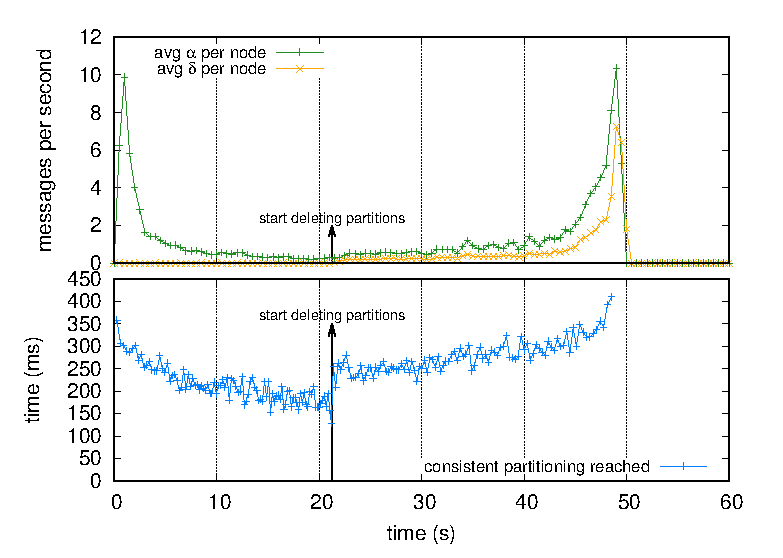
\includegraphics[width=0.99\columnwidth]{img/as_cast_complexity.eps}
  \caption{\label{fig:complexity}Overhead of, and time before,
    reaching consistent partitioning using \NAME.}
  %% \caption{\label{fig:complexity}Cumulative average number of messages
  %%   per process in a network comprising 10k processes; along with the
  %%   duration before reaching consistent partitioning after adding or
  %%   removing a partition, totaling 100 new partition then removed.}
\end{figure}

\item [Results:]

Figure~\ref{fig:complexity} shows the results of this experiment. The
top part of the figure shows the average traffic per process divided
between $\alpha$ and $\delta$ messages. The bottom part of the figure
shows the time before reaching consistent partitioning.

\noindent Figure~\ref{fig:complexity} confirms that \NAME's overhead
depends on the size of partitions. The first partition is the most
expensive, for $\alpha$'s must reach every process which takes time
and generate more traffic. Still, being reactive, as opposed as
cycle-based protocols~\cite{jelasity2007gossip}, \NAME quickly
converge towards consistent partitioning in only 350 milliseconds. The
last and $100^{th}$ partition added around 21 seconds is the least
expensive. By using scoped broadcast, control information only reaches
a small subset of the whole network.

\noindent Figure~\ref{fig:complexity} also confirms that \NAME's
delete operations are more expensive than add operations. Indeed, the
top part of the figure shows that after 21 seconds, when the
experiment involves removals, traffic includes both $\alpha$'s and
$\delta$'s. The latter aims at removing stale information and
triggering competition while the former aims at updating shortest
paths. As corollary, the convergence time increases, for $\delta$'s
must reach every partition border before any sound competitors
propagate their partition. It is worth noting that this delete
operation involves concurrency: removals continue to propagate while
the competition is already partially triggered and propagating.

\noindent Figure~\ref{fig:complexity} shows that the overhead of
adding the $1^{st}$ partition does not correspond to the overhead of
deleting this $1^{st}$ partition. When adding it, messages must reach
all processes while when removing it, messages must reach a small
subset of this membership. This is important, for it means that
\NAME's overhead actually depends on the current partitioning, and
does not depend on the past partitioning.

\noindent Finally, Figure~\ref{fig:complexity} highlights that after
49 seconds, i.e., after the 100 adds and the 100 deletes, processes do
not generate traffic anymore. Being reactive, \NAME has no overhead
when there is no operation in the system. This is important, for it
means that \NAME's overhead actually depends on its usage.

\end{asparadesc}

\subsection{Distribution and hotspots}


\subsection{Inter-autonomous systems}

% \subsection{Use case: caching}
% \subsection{Use case: routing}
% \subsection{Use case: broadcast domain}


%%% Local Variables: 
%%% mode: latex
%%% TeX-master: "../paper"
%%% ispell-local-dictionary: "english"
%%% End: 


\section{Related Work}
\label{sec:related_work}

Content indexing services in geo-distributed infrastructures allow
\processes to retrieve specific content while leveraging the
advantages of replication. These systems mostly rely on dedicated
location services hosted by possibly remote third-party \processes; but
cutting out the middleman requires that each \process maintains its
own index in a decentralized fashion.
% This section reviews these
% approaches.

\begin{asparadesc}
\item [Third-party:]

Dedicated services possibly hosted by remote third-party \processes
are popular, for they propose the simplest mean to deploy such a
service. They must maintain
\begin{inparaenum}[(i)]
\item the list of current replicas along with their respective
  location; and
\item the network topology to determine the closest replica for every
  requesting \process.
\end{inparaenum}

\noindent A central server that registers both these information
facilitates the computation, for it gathers all knowledge in one
place~\cite{snamp, p2p-oracle, fogstore, p2p-alto}. However, it comes with
well-known issues such as load balancing, or single point of failure.
%% Numerous solutions
%% maintain an index of all replica locations on a centralized
%% server. This comes with well-known disadvantages inherent to
%% centralized solutions such as load balancing, robustness or locality
%% that are even magnified in an Edge context.

\noindent Distributing this index among \processes circumvents these
issues~\cite{voronet, ipfs, mdht, squirrel, coin_19}, but still raises
locality issues where \processes
\begin{inparaenum}[(i)]
\item request to a possibly far away location service the content
  location, and then
\item request the actual content from far away replicas.
\end{inparaenum}
For instance, using \underline{d}istributed \underline{h}ash
\underline{t}ables (DHT)~\cite{ipfs, mdht, squirrel}, each \process
stores a part of the index defined by an interval between hash values.
The hash values are the keys to retrieve the associated content
location.  Before downloading any content, a \node asks for its
location using its key. After a series of round-trips between DHT
servers possibly distant from each other, the \node gets a list of
available replicas. Contrarily to \NAME, such services do not ensure
to include the closest replica.

\noindent In addition, they often do not include distance information
along with replica location. Determining where resides the closest
replica for every requesting \process necessarily involves some
knowledge about the \emph{current} topology.  Maintaining a consistent
view of an ever changing topology across a network is inherently
complicated~\cite{topology-discovery, ospf}.
%%  As for the index, this knowledge about the topology can be either
%% centralized~\cite{topology-discovery} or distributed like in
%% routing protocols such as \underline{O}pen \underline{S}hortest
%% \underline{P}ath \underline{F}irst (OSPF)~\cite{ospf}.
As a consequence, the requesting \node ends up downloading from multiple
replica hosts, yet only keeping the fastest answer. \Processes either
waste network resources, or face lower response time.

% We emphasize that, in this setting, the DHT only stores information
% about replicas locations, not the content itself.

%% Distributing this index among \processes in the network circumvent
%% some of these issues, either using coordinate-based
%% overlays~\cite{voronet, coin_19} or \underline{D}istributed
%% \underline{H}ash \underline{T}ables (DHTs)~\cite{ipfs, mdht,
%%   squirrel}. In the latter, each node stores a part of the index,
%% defined by an interval between hash values.  Before downloading any
%% object, a node first hashes the content to obtain the address of the
%% node that stores the replica locations of this given object. After
%% obtaining from the remote node the list of available replicas, it can
%% select the closest copy to download from. We emphasize that, in this
%% setting, the DHT only stores information about replicas locations, not
%% the content itself.



%% \noindent All the aforementionned solutions require to contact a remote node to
%% request this index which is costly in terms of latency while in
%% contradiction with Edge infrastructure constraints, as previously
%% explained.


\item [Fully decentralized:]

Cutting out the middleman by hosting a location service on each and
every \process improves response time of content retrieval. However,
it still requires every \process to index every live replica as well
as their respective distance in order to rank them.
%% The opposite approach consists in hosting the index directly on the
%% nodes, avoiding any prior request to access a content.
\underline{N}amed \underline{D}ata \underline{N}etworking
(NDN)~\cite{nlsr} broadcasts information about cache updates to all
\nodes in the system. Having the entire knowledge of all the replica
locations along with distance information carried into messages, each
\node easily determine where the closest copy of specific content
resides, without contacting any remote
service. \underline{C}onflict-\underline{f}ree \underline{r}eplicated
\underline{d}atatype (CRDT)~\cite{shapiro2011crdts} for set data
structures could also implement such a location service. \Processes
would eventually have a set of all replicas, assuming eventual
delivery of messages.
\noindent Such solutions imply that every \process receives every
message, which contradicts the principles of Edge infrastructures that
aim at reducing the volume of data passing through the network. On the
opposite, each \process running \NAME only registers its closest
replica. This allows \NAME to use scoped broadcast as a communication
primitive to lock down the traffic generated by content indexing based
on distances.
% Such solutions inherently imply that every node will
% eventually receive all messages, contrary to \NAME.

\item [Scoped flooding:]

Some state-of-the-art approaches confine the dissemination of messages
to interested \processes too.
% \item [Membership protocols:]

\noindent Distance-based membership protocols such as
T-Man~\cite{t-man} make \processes converge to a specific network
topology depending on targeted properties. They periodically
communicate with their neighbors to compare their state. Following
this exchange, they add and remove communication links to other
\processes. Over exchanges, they converge towards a topology ensuring
the targeted properties.  While at first glance membership protocols
and \NAME could share common preoccupations, \NAME does not aim at
building any topology and never modifies neighbors of \processes.

%% In
%% addition, distance-based membership protocols often rely on random
%% peer-sampling protocols to avoid falling in a local minimum that would
%% stop them from reaching this targeted topology. This contradicts with
%% the principles of Edge infrastructures as well, in a minor way.

%% At first glance, membership protocols~\cite{t-man} would appear to
%% provide suitable abstractions to create a scope-related
%% partitioning, as proposed in this paper. Such protocols usually
%% rely on gossip mechanisms, implying contacts with random nodes that
%% can be far away in the physical topology.  They are mostly
%% implemented by modifying the neighboring of a given node according
%% to a certain metric in a logical overlay.

%% These protocols are usually cycle-based, meaning that they impose a
%% constant load on the network traffic, even when the system state does
%% not change. \NAME only generates traffic upon system changes.

\noindent The most closely related approaches to \NAME come from
\underline{i}nformation-\underline{c}entric \underline{n}etworking
(ICN)~\cite{garcia-lopez, hemmati2015namebased}. They periodically
advertise their cache content, and advertisements stop as soon as they
reach uninterested \processes. However their operation requires that
\begin{inparaenum}[(i)]
\item they constantly generate traffic even in quiescent systems where
  \processes do not add nor destroy replicas; and 
\item they define physical-clock-based timeouts the value of which
  depends on network topology properties such as network diameter.
  %also incur an overhead even in quiet contexts without any update.
  % Moreover, they necessarily rely on physical timeouts
  Unfitting timeouts lead to premature removals of live replicas; or
  slow convergence where \processes wrongly believe that their closest
  replica is live while it was destroyed.
\end{inparaenum}
On the opposite, \NAME quickly informs each \process of its closest
replica even in large networks; and when the system becomes quiescent,
\NAME has no overhead.

\end{asparadesc}

%Finally, we emphasize that consistency is at the core of our design,
%as \NAME provides the same guarantees for all nodes.  On the
%contrary, to avoid flooding, authors in~\cite{opnl} propose to
%propagate information about cache updates only towards the original
%replica. This enables for a request to be caught \textit{on-path},
%and be redirected to the closest replica. However, the announcement
%is only performed towards this original replica, that is requests can
%miss closer replicas that are not on this path, thus decreasing the
%efficiency of the cache sharing mechanism.

%AVK: This should go where we explain the DEL, as this is really
%specific...  One could also solve this issue by removing partitions
%that were not advertised for a defined
%time~\cite{hemmati2015namebased, garcia-lopez}.  However, relying on
%physical timeout could lead to either premature removals of
%partitions when they are still operating; or slow convergence where
%processes believe they belong to a partition that was removed
%(\TODO{plot ?}). In addition, since timeouts imply a continuous
%maintenance of partitions, such partitioning protocol incurs an
%overhead even in quiet contexts without dynamic partitions.


% AVK t-man: T-Man: Gossip-Based Overlay Topology Management5doat a
% random time at a random time once in eachconsecutive interval of T
% time unit This buffer contains a random sample of the nodes from the
% entirenetwork. It is provided by apeer sampling service We do not
% try to to create a topology aware overlay ! Because locality.  We do
% not provide routing ! routing is two determine path between any pair
% of nodes. We only provide path to objects Koala locality aware
% routing. Long links. Lazzy (nothing happens) Koala shares many core
% aspectswith similar overlays, such as Chord and Symphony.  VoroNet:
% overlay and routing. i.e. long links It links application objects
% rathen than physical nodes so that objects with similar
% characteristic are neighbors.  are logigal overlay, that are not
% correlated to the physical infrstructure.  Usually rely on long
% links...  AVK

%%% Local Variables: 
%%% mode: latex
%%% TeX-master: "../paper"
%%% ispell-local-dictionary: "english"
%%% End: 


\section{Conclusion}
\label{sec:conclusion}

With the advent of the Edge and IoT era, major distributed services
proposed by our community should be revised to mitigate as much as
possible traffic between \processes.  In this paper, we addressed the
challenge of content indexing as a dynamic logical partitioning
problem where partitions grow and shrink to reflect content and
replicas locations, as well as infrastructure changes.  Using an
efficient communication primitive called scoped broadcast, each
\process composing the infrastructure eventually knows the \process
hosting the best replica of a specific content.  The challenge resides
in handling concurrent operations that may impair the propagation of
messages, and in turn, lead to inconsistent partitioning.
%% The major difficulty lies in concurrent operations, each having a
%% different scope, and ensure the correct convergence of the system.  We
%% defined, in particular, multiple properties that highlight this
%% complexity.
%
We highlighted the properties that solve this problem and proposed an
implementation called \NAME.  Our simulations confirmed that
\processes quickly reach consistent partitioning together, and that
the generated traffic remains locked down to partitions.  We also
briefly discussed \NAMEC, an improvement to contain the traffic in relevant
autonomous systems.
%% correctness of our protocol as well as the confinement of
%% the traffic only where it is needed.

%% As future work, we plan to leverage the hierarchical properties of
%% interconnected autonomous systems to further limit the propagation of
%% indexes within interested systems only. We expect that such an
%% improvement would greatly benefit the autonomous systems, and
%% particularly those hosting a large number of contents.

%% Systems hosting a large number of contents would greatly benefit from
%% this improvement.

%% As future work, we plan to enable lazy retrieval of partitions when a
%% large number of contents is involved. Indeed, using \NAME, every
%% \process partakes in the propagation of all indexes which raises
%% scalability issues. We would like to leverage the hierarchical
%% properties of
%% % interconnected
%% autonomous systems to limit the
%% propagation of such indexes only to interested systems.

%
%% As ongoing and future work, we are currently studying how it might be
%% possible to limit the scope of a partition to one autonomous system at
%% most. Indeed, the gain of propagating changes to \processes belonging to
%% another autonomous system might be negligible as the latency penalty
%% is mainly due to inter autonomous systems' links (\eg trans-continental
%% links).  Exactly, we are investigating how such a change can be
%% formalized and its impact on the current protocol.
%
%autonomous systems. Indeed, \processes could leverage the hierarchical
%properties of the Internet topology~\cite{nur2018geography} to avoid
%flooding the whole systems with control information about all
%partitions.
%\TODO{should we highlight this at the end of the experiment}
%

At mid-term, we plan to evaluate our proposal within a concrete
storage system such as \underline{I}nter\underline{P}lanetary
\underline{F}ile \underline{S}ystem
(IPFS)~\cite{ipfs}. This would allow us to assess the
relevance of the \NAME approach in a real system subject to high
dynamicity, and compare it against its current DHT-based indexing
system that does not include distance in its operation. More generally,
we claim \NAME (or \NAMEC) can constitute a novel building block for
geo-distributed services.  Among the use-cases we have identified,
\NAME can be used to complement content delivery infrastructures by
efficiently sharing between \process attached to the same CDN server
the locatiosn of web objects that have been already downloaded. This
would allow the containment of web traffic even lower in our networks,
and so reduce the overall traffic footprint.


%% Such an integration would enable us to to perform additional
%% experiments and observe the gain with respect to the DHT-based
%% approach that is currently used.

%% In addition to this action, it would make sense to evaluate
%% the use of \NAME within a concrete storage systems, such as
%% \underline{I}nter\underline{P}lanetary \underline{F}ile
%% \underline{S}ystem (IPFS)~\cite{henningsen2020mapping}.  Such an
%% integration would enable us to to perform additional experiments and
%% observe the gain with respect to the DHT-based approach that is
%% currently used.

%
%% More generally, it can be used in other services in order to share information while mitigating the traffic.
%% MWhile we use the distance to the closest copy in this paper, It is
%% notewothy that other scopes can be envisioned according to the
%% use-cases.  For instance, the location of a city in order to broadcast
%% message to all nodes in the city.  This requires nodes to store and
%% maintain their city location in their local state. Nodes stop
%% delivering and forwarding their received messages when they come from
%% a different city. Such a predicate can be complexified in order to
%% broadcast messages to all nodes in the city plus neighboring
%% cities. This requires nodes to overload forwarded messages the first
%% time they reach another city. The predicate checks if messages already
%% reached two distinct cities before delivery.  The predicate can even
%% be piggypack within the message and so be different for each
%% message.\TODO{Complete the use-cases}





%%% Local Variables: 
%%% mode: latex
%%% TeX-master: "../paper"
%%% ispell-local-dictionary: "english"
%%% End: 

%% \input{input/acknowledgment.tex}

\bibliographystyle{plainurl}
\bibliography{compact_bibliographie}
  
\end{document}

%%% Local Variables:
%%% mode: latex
%%% ispell-local-dictionary: "english"
%%% End:
